\documentclass[12pt]{article}

% Packages for math, graphics, and layout
\usepackage{amsmath,amssymb,amsthm}
\usepackage{mathtools}
\usepackage{graphicx}
\usepackage{float}
\usepackage{hyperref}
\usepackage{xcolor}
\usepackage{listings}
\usepackage{geometry}
\usepackage{algorithm}
\usepackage{algpseudocode}
\usepackage{tikz}
\usepackage{longtable}
\usepackage{circuitikz}
\usepackage{comment}
\usepackage{MnSymbol}
\usepackage{physics}
\usepackage{booktabs}
\usepackage[section]{placeins}
\usepackage{karnaugh-map}

% Additional packages for improved header and spacing
\usepackage{fancyhdr}
\usepackage{titlesec}
\usepackage{setspace}

% Custom commands
\newcommand*\xor{\oplus}

% Page geometry and header settings
\geometry{a4paper, margin=1in}
\pagestyle{fancy}
\fancyhf{}
\fancyhead[L]{BCD Counter with T Flip-Flops}
\fancyhead[R]{EE24BTECH11002 EE24BTECH11024}
\fancyfoot[C]{\thepage}

% Title setup
\title{\textbf{BCD Counter with T Flip-Flops}}
\author{\textbf{EE24BTECH11002 EE24BTECH11024}}
\date{\today}

% Adjust section spacing for a cleaner look
\titlespacing*{\section}{0pt}{1.5ex plus 1ex minus .2ex}{1ex}
\titlespacing*{\subsection}{0pt}{1.2ex plus .8ex minus .2ex}{0.8ex}

\begin{document}
\maketitle
\thispagestyle{fancy}

\begin{abstract}
This document details the design and implementation of a bidirectional BCD counter using T flip-flops. The counter, which counts from 0 to 9 (and vice versa), employs additional logic to skip invalid BCD states. The design includes detailed state tables, Karnaugh maps, and circuit diagrams.
\end{abstract}

\section*{Aim}
To design and implement a BCD (Binary Coded Decimal) counter using T flip-flops that can count both up and down based on input conditions, with a maximum count of 9 (0--9).

\section*{Apparatus}
\begin{itemize}
    \item JK Flip-Flops (IC 7476) configured as T flip-flops (by tying J and K high) -- 4 units
    \item Logic gates (AND, OR, XOR, NOT gates)
    \item Push buttons (2 units -- one for up counting, one for down counting)
    \item 7-segment display with BCD to 7-segment decoder
    \item Power supply (5V DC)
    \item Breadboard and jumper wires
    \item Resistors (1k$\Omega$, 330$\Omega$)
    \item Arduino board (for clock generation and power)
    \item Oscilloscope (to verify clock signals)
    \item Logic analyzer (to verify state transitions)
\end{itemize}

\section*{Theory}
A BCD counter is a digital counter that counts from 0 (0000) to 9 (1001) in binary and then resets back to 0. In this experiment, we implement a bidirectional BCD counter using T flip-flops that can count both up and down based on input signals.

\subsection*{T Flip-Flop}
T flip-flops (Toggle flip-flops) change their output state when triggered by a clock pulse if their T input is 1. If \(T=0\), the output remains unchanged. This makes them ideal for counter applications.

The characteristic equation of a T flip-flop is:
\[
Q^+ = Q \oplus T
\]
where:
\begin{itemize}
    \item \(Q^+\) is the next state,
    \item \(Q\) is the current state,
    \item \(T\) is the toggle input,
    \item \(\oplus\) represents the XOR operation.
\end{itemize}

A T flip-flop can be constructed from a JK flip-flop by connecting both J and K inputs to the same signal \(T\). When \(T=1\), the flip-flop toggles on each clock pulse; when \(T=0\), it maintains its state.

\subsection*{BCD Counter}
A BCD counter counts from 0 to 9 in binary (0000 to 1001) and then resets to 0. Since a 4-bit binary counter can represent 16 states (0--15), additional logic is required to skip the invalid states (10--15). This counter is known as a modulo-10 counter.

\subsection*{7-Segment Display}
The 7-segment display consists of seven LEDs arranged in a pattern to display decimal digits. A BCD-to-7-segment decoder converts the 4-bit BCD output from the counter into signals that illuminate the appropriate segments (labeled 'a' through 'g') to display digits 0--9.

\section*{Derivation of Logic}

Below are the state tables and Karnaugh map derivations for both the up and down counter modes.

\subsection*{State Tables}

\textbf{Up Counter State Table:}
\begin{table}[H]
\centering
\begin{tabular}{|c|c|c|c||c|c|c|c||c|c|c|c|}
\hline
\multicolumn{4}{|c||}{Present State} & \multicolumn{4}{c||}{T Flip-Flops} & \multicolumn{4}{c|}{Next State} \\
\hline
\(Q_3\) & \(Q_2\) & \(Q_1\) & \(Q_0\) & \(T_3\) & \(T_2\) & \(T_1\) & \(T_0\) & \(Q_3\) & \(Q_2\) & \(Q_1\) & \(Q_0\) \\
\hline
0 & 0 & 0 & 0 & 0 & 0 & 0 & 1 & 0 & 0 & 0 & 1 \\
\hline
0 & 0 & 0 & 1 & 0 & 0 & 1 & 1 & 0 & 0 & 1 & 0 \\
\hline
0 & 0 & 1 & 0 & 0 & 0 & 0 & 1 & 0 & 0 & 1 & 1 \\
\hline
0 & 0 & 1 & 1 & 0 & 1 & 1 & 1 & 0 & 1 & 0 & 0 \\
\hline
0 & 1 & 0 & 0 & 0 & 0 & 0 & 1 & 0 & 1 & 0 & 1 \\
\hline
0 & 1 & 0 & 1 & 0 & 0 & 1 & 1 & 0 & 1 & 1 & 0 \\
\hline
0 & 1 & 1 & 0 & 0 & 0 & 0 & 1 & 0 & 1 & 1 & 1 \\
\hline
0 & 1 & 1 & 1 & 1 & 1 & 1 & 1 & 1 & 0 & 0 & 0 \\
\hline
1 & 0 & 0 & 0 & 0 & 0 & 0 & 1 & 1 & 0 & 0 & 1 \\
\hline
1 & 0 & 0 & 1 & 1 & 0 & 0 & 1 & 0 & 0 & 0 & 0 \\
\hline
1 & 0 & 1 & 0 & X & X & X & X & X & X & X & X \\
\hline
1 & 0 & 1 & 1 & X & X & X & X & X & X & X & X \\
\hline
1 & 1 & 0 & 0 & X & X & X & X & X & X & X & X \\
\hline
1 & 1 & 0 & 1 & X & X & X & X & X & X & X & X \\
\hline
1 & 1 & 1 & 0 & X & X & X & X & X & X & X & X \\
\hline
1 & 1 & 1 & 1 & X & X & X & X & X & X & X & X \\
\hline
\end{tabular}
\caption{State table for the single-digit BCD Up-counter. (X denotes don't-care conditions.)}
\end{table}

\vspace{0.5cm}
\textbf{Down Counter State Table:}
\begin{table}[H]
\centering
\begin{tabular}{|c|c|c|c||c|c|c|c||c|c|c|c|}
\hline
\multicolumn{4}{|c||}{Present State} & \multicolumn{4}{c||}{T Flip-Flops} & \multicolumn{4}{c|}{Next State} \\
\hline
\(Q_3\) & \(Q_2\) & \(Q_1\) & \(Q_0\) & \(T_3\) & \(T_2\) & \(T_1\) & \(T_0\) & \(Q_3\) & \(Q_2\) & \(Q_1\) & \(Q_0\) \\
\hline
0 & 0 & 0 & 0 & 1 & 0 & 0 & 1 & 1 & 0 & 0 & 1 \\
\hline
0 & 0 & 0 & 1 & 0 & 0 & 0 & 1 & 0 & 0 & 0 & 0 \\
\hline
0 & 0 & 1 & 0 & 0 & 0 & 1 & 1 & 0 & 0 & 0 & 1 \\
\hline
0 & 0 & 1 & 1 & 0 & 0 & 0 & 1 & 0 & 0 & 1 & 0 \\
\hline
0 & 1 & 0 & 0 & 0 & 1 & 1 & 1 & 0 & 0 & 1 & 1 \\
\hline
0 & 1 & 0 & 1 & 0 & 0 & 0 & 1 & 0 & 1 & 0 & 0 \\
\hline
0 & 1 & 1 & 0 & 0 & 0 & 1 & 1 & 0 & 1 & 0 & 1 \\
\hline
0 & 1 & 1 & 1 & 0 & 0 & 0 & 1 & 0 & 1 & 1 & 0 \\
\hline
1 & 0 & 0 & 0 & 1 & 1 & 1 & 1 & 0 & 1 & 1 & 1 \\
\hline
1 & 0 & 0 & 1 & 0 & 0 & 0 & 1 & 1 & 0 & 0 & 0 \\
\hline
1 & 0 & 1 & 0 & X & X & X & X & X & X & X & X \\
\hline
1 & 0 & 1 & 1 & X & X & X & X & X & X & X & X \\
\hline
1 & 1 & 0 & 0 & X & X & X & X & X & X & X & X \\
\hline
1 & 1 & 0 & 1 & X & X & X & X & X & X & X & X \\
\hline
1 & 1 & 1 & 0 & X & X & X & X & X & X & X & X \\
\hline
1 & 1 & 1 & 1 & X & X & X & X & X & X & X & X \\
\hline
\end{tabular}
\caption{State table for the single-digit BCD Down-counter. (X denotes don't-care conditions.)}
\end{table}

\newpage
\subsection*{Karnaugh Maps for T Flip-Flops}

\subsubsection*{Up Counter T Flip-Flops}
\textbf{For \(T_0\):}\\
Since \(T_0 = 1\) for all cases, no Karnaugh map is required.

\vspace{0.5cm}
\textbf{For \(T_1\):}
\begin{center}
\begin{karnaugh-map}[4][4][1][$Q_1Q_0$][$Q_3Q_2$]
\manualterms{0,1,0,1,0,1,0,1,0,0,X,X,X,X,X,X}
\implicant{1}{7}
\end{karnaugh-map}
\end{center}
Thus, 
\[
T_1 = \overline{Q_3}\,Q_0.
\]

\vspace{0.3cm}
\textbf{For \(T_2\):}
\begin{center}
\begin{karnaugh-map}[4][4][1][$Q_1Q_0$][$Q_3Q_2$]
\manualterms{0,0,0,1,0,0,0,1,0,0,X,X,X,X,X,X}
\implicant{3}{11}
\end{karnaugh-map}
\end{center}
Thus, 
\[
T_2 = Q_1\,Q_0.
\]

\vspace{0.5cm}
\textbf{For \(T_3\):}
\begin{center}
\begin{karnaugh-map}[4][4][1][$Q_1Q_0$][$Q_3Q_2$]
\manualterms{0,0,0,0,0,0,0,1,0,1,X,X,X,X,X,X}
\implicant{13}{11}
\implicant{7}{15}
\end{karnaugh-map}
\end{center}
Thus, 
\[
T_3 = Q_2\,Q_1\,Q_0 + Q_3\,Q_0.
\]

\subsubsection*{Down Counter T Flip-Flops}
\textbf{For \(T_0\):}\\  
Again, \(T_0 = 1\) for all cases.

\vspace{0.5cm}
\textbf{For \(T_1\):}
\begin{center}
\begin{karnaugh-map}[4][4][1][$Q_1Q_0$][$Q_3Q_2$]
\manualterms{0,0,1,0,1,0,1,0,1,0,X,X,X,X,X,X}
\implicant{2}{10}
\implicant{4}{12}
\implicant{12}{8}
\end{karnaugh-map}
\end{center}
Thus,
\[
T_1 = Q_1\,\overline{Q_0} + Q_2\,\overline{Q_1}\,\overline{Q_0} + Q_3\,\overline{Q_1}\,\overline{Q_0}.
\]

\vspace{0.5cm}
\textbf{For \(T_2\):}
\begin{center}
\begin{karnaugh-map}[4][4][1][$Q_1Q_0$][$Q_3Q_2$]
\manualterms{0,0,0,0,1,0,0,0,1,0,X,X,X,X,X,X}
\implicant{4}{12}
\implicant{12}{8}
\end{karnaugh-map}
\end{center}
Thus,
\[
T_2 = Q_2\,\overline{Q_1}\,\overline{Q_0} + Q_3\,\overline{Q_1}\,\overline{Q_0}.
\]

\vspace{0.5cm}
\textbf{For \(T_3\):}
\begin{center}
\begin{karnaugh-map}[4][4][1][$Q_1Q_0$][$Q_3Q_2$]
\manualterms{1,0,0,0,0,0,0,0,1,0,X,X,X,X,X,X}
\implicantedge{0}{0}{8}{8}
\end{karnaugh-map}
\end{center}
Thus,
\[
T_3 = \overline{Q_2}\,\overline{Q_1}\,\overline{Q_0}.
\]
The Karnaugh maps for Down counter can be simplified further but the reason to leave them as give is, take $T = \overline{Q_1}\,\overline{Q_0}$ then:
\begin{enumerate}
    \item $T_0 = 1$
    \item $T_1 = Q_1\,\overline{Q_0} + T_2$
    \item $T_2 = (Q_1 + Q_2)T$
    \item $T_3 = \overline{Q_2}\,T$
\end{enumerate}
Which are easier to make in Circuit

\newpage

\section*{Converting JK Flip flop to T Flip flop}
A JK Flip-Flop can be configured as a T Flip-Flop by connecting both J and K inputs to the same signal (T). When J=K=1, the flip-flop toggles with each clock pulse, which is the behavior of a T flip-flop with T=1.

\begin{figure}[!ht]
\centering
\resizebox{0.6\textwidth}{!}{%
\begin{circuitikz}
\tikzstyle{every node}=[font=\LARGE]

\draw  (4.25,12.5) rectangle (8.75,7.75);
\draw (4.25,11.5) to[short] (2.75,11.5);
\node at (4.25,11.5) [circ] {};
\node at (4.25,8.75) [circ] {};
\node at (8.75,11.5) [circ] {};
\node at (8.75,8.75) [circ] {};
\node [font=\LARGE] at (4.75,11.5) {J};
\node [font=\LARGE] at (4.75,10.25) {K};
\draw (4.25,10.25) to[short] (2.75,10.25);
\node at (4.25,10.25) [circ] {};
\draw (4.25,9.25) to[short] (4.75,8.75);
\draw (4.75,8.75) to[short] (4.25,8.25);
\node [font=\LARGE] at (5.5,8.75) {CLK};
\node [font=\LARGE] at (8.25,11.5) {Q};
\node [font=\LARGE] at (8.25,8.75) {Q'};
\draw (2.75,11.5) to[short] (2.75,10.25);
\draw (2.75,11) to[short] (1.25,11);
\node [font=\LARGE] at (0.75,11) {T};
\draw (4.25,8.75) to[short] (1.25,8.75);
\draw [ dashed] (2,13.25) rectangle  (10.75,7.25);
\draw (8.75,11.5) to[short] (12,11.5);
\draw (8.75,8.75) to[short] (12,8.75);
\end{circuitikz}
}%
\caption{Constructing T Flipflop using JK Flipflop}
\end{figure}
\FloatBarrier

\section*{Circuit Diagram}

\subsection*{Circuit Diagram for Incrementing}
\begin{figure}[!ht]
\centering
\resizebox{1\textwidth}{!}{%
\begin{circuitikz}
\tikzstyle{every node}=[font=\LARGE]
\draw  (5,15.75) rectangle (8.75,10.75);
\draw  (11.25,15.75) rectangle (15,10.75);
\draw  (17.5,15.75) rectangle (21.25,10.75);
\draw  (-1.25,15.75) rectangle (2.5,10.75);
\node [font=\LARGE] at (-0.5,15) {$T_0$};
\node [font=\LARGE] at (-0.5,11.25) {Clk};
\node [font=\LARGE] at (2,14.5) {$Q_0$};
\node [font=\LARGE] at (2,12) {$Q_0$};
\draw (1.5,12.5) to[short] (2.25,12.5);
\node [font=\LARGE] at (5.75,15) {$T_1$};
\node [font=\LARGE] at (8.25,14.5) {$Q_1$};
\node [font=\LARGE] at (8.25,12) {$Q_1$};
\draw (7.75,12.5) to[short] (8.5,12.5);
\node [font=\LARGE] at (5.75,11.25) {Clk};
\node [font=\LARGE] at (12,15) {$T_2$};
\node [font=\LARGE] at (14.5,14.5) {$Q_2$};
\node [font=\LARGE] at (14.5,12) {$Q_2$};
\draw (14,12.5) to[short] (14.75,12.5);
\node [font=\LARGE] at (12,11.25) {Clk};
\node [font=\LARGE] at (18.25,15) {$T_3$};
\node [font=\LARGE] at (20.75,14.5) {$Q_3$};
\node [font=\LARGE] at (20.75,12) {$Q_3$};
\draw (20.25,12.5) to[short] (21,12.5);
\node [font=\LARGE] at (18.25,11.25) {Clk};
\draw (-6.25,9.5) to[short] (-2.5,9.5);
\draw (-2.5,9.5) to[short] (-2.5,11.5);
\draw (-2.5,11.5) to[short] (-1.25,11.5);
\draw (-2.5,9.5) to[short] (3.75,9.5);
\draw (3.75,9.5) to[short] (3.75,11.5);
\draw (3.75,11.5) to[short] (5,11.5);
\draw (3.75,9.5) to[short] (10,9.5);
\draw (10,9.5) to[short] (10,11.5);
\draw (10,11.5) to[short] (11.25,11.5);
\draw (10,9.5) to[short] (16.25,9.5);
\draw (16.25,9.5) to[short] (16.25,11.5);
\draw (16.25,11.5) to[short] (17.5,11.5);
\draw (-1.25,15) to[short] (-2,15);
\draw (-2,15) to[battery1] (-2,16.5);
\draw (-2,16.5) to (-3,16.5) node[ground]{};
\draw (21.25,12) to[short] (22.5,12);
\draw (22.5,12) to[short] (23.25,12);
\draw (23.25,12) to[short] (23.25,16.5);
\draw (23.25,16.5) to[short] (7,16.5);
\draw (2.5,14.5) to[short] (3,14.5);
\draw (7,17) to[short] (6.75,17);
\draw (7,16.5) to[short] (6.75,16.5);
\draw (6.75,17) node[ieeestd and port, anchor=in 2, scale=0.89, rotate=180](port){} (port.out) to[short] (4.75,16.75);
\draw (3,14.5) to[short] (3,18);
\draw (3,18) to[short] (7,18);
\draw (7,18) to[short] (7,17);
\draw (4.75,16.75) to[short] (4.25,16.75);
\draw (4.25,16.75) to[short] (4.25,15);
\draw (4.25,15) to[short] (5,15);
\draw (8,18.25) to[short] (8.5,18.25);
\draw (8,17.75) to[short] (8.5,17.75);
\draw (8.5,18.25) node[ieeestd and port, anchor=in 1, scale=0.89](port){} (port.out) to[short] (10.75,18);
\draw (8.75,14.5) to[short] (9.25,14.5);
\draw (9.25,14.5) to[short] (9.25,16.75);
\draw (9.25,16.75) to[short] (8,16.75);
\draw (8,16.75) to[short] (8,17.75);
\draw (8,18.25) to[short] (7,18.25);
\draw (7,18.25) to[short] (7,17.75);
\draw (10.75,18) to[short] (10.75,15);
\draw (10.75,15) to[short] (11.25,15);
\draw (16.25,18.75) to[short] (16.5,18.75);
\draw (16.25,18.25) to[short] (16.5,18.25);
\draw (16.5,18.75) node[ieeestd or port, anchor=in 1, scale=0.89](port){} (port.out) to[short] (18.25,18.5);
\draw (13.25,19.5) to[short] (13.5,19.5);
\draw (13.25,19) to[short] (13.5,19);
\draw (13.5,19.5) node[ieeestd and port, anchor=in 1, scale=0.89](port){} (port.out) to[short] (15.25,19.25);
\draw (13.25,17.75) to[short] (13.5,17.75);
\draw (13.25,17.25) to[short] (13.5,17.25);
\draw (13.5,17.75) node[ieeestd and port, anchor=in 1, scale=0.89](port){} (port.out) to[short] (15.25,17.5);
\draw (16.75,17) to[short] (16.75,15);
\draw (16.75,15) to[short] (17.5,15);
\draw (21.25,14.5) to[short] (22,14.5);
\draw (22,14.5) to[short] (22,20.75);
\draw (22,20.75) to[short] (13.25,20.75);
\draw (13.25,20.75) to[short] (13.25,19.5);
\draw (7,18.25) to[short] (7,19);
\draw (7,19) to[short] (13.25,19);
\draw (15,14.5) to[short] (15.5,14.5);
\draw (15.5,14.5) to[short] (15.5,16.25);
\draw (15.5,16.25) to[short] (13.25,16.25);
\draw (13.25,16.25) to[short] (13.25,17.25);
\draw (10.75,17.75) to[short] (13.25,17.75);
\node [font=\LARGE] at (-6.75,9.5) {Clk};
\draw (15.25,19.25) to[short] (15.75,19.25);
\draw (15.75,19.25) to[short] (15.75,18.75);
\draw (15.75,18.75) to[short] (16.25,18.75);
\draw (15.25,17.5) to[short] (15.75,17.5);
\draw (15.75,17.5) to[short] (15.75,18.25);
\draw (15.75,18.25) to[short] (16.25,18.25);
\draw (18.25,18.5) to[short] (18.75,18.5);
\draw (18.75,18.5) to[short] (18.75,17);
\draw (18.75,17) to[short] (16.75,17);
\end{circuitikz}
}%

\caption{Circuit diagram representing the logic for incrementing.}
\label{fig:Incrementing}
\end{figure}

Let the circuit be represented as:

\begin{figure}[!ht]
\centering
\resizebox{1\textwidth}{!}{%
\begin{circuitikz}
\tikzstyle{every node}=[font=\LARGE]
\draw  (-3.75,15.75) rectangle (0,13.25);
\draw  (2.5,15.75) rectangle (6.25,13.25);
\draw  (8.75,15.75) rectangle (12.5,13.25);
\draw  (15,15.75) rectangle (18.75,13.25);
\node [font=\LARGE] at (-3,15.25) {$T_0$};
\node [font=\LARGE] at (-3,13.75) {Clk};
\node [font=\LARGE] at (-0.5,14.5) {$Q_0$};
\node [font=\LARGE] at (3.25,15.25) {$T_1$};
\node [font=\LARGE] at (3.25,13.75) {Clk};
\node [font=\LARGE] at (5.75,14.5) {$Q_1$};
\node [font=\LARGE] at (9.5,15.25) {$T_2$};
\node [font=\LARGE] at (9.5,13.75) {Clk};
\node [font=\LARGE] at (12,14.5) {$Q_2$};
\node [font=\LARGE] at (15.75,15.25) {$T_3$};
\node [font=\LARGE] at (15.75,13.75) {Clk};
\node [font=\LARGE] at (18.25,14.5) {$Q_3$};
\draw  (3.75,9.5) rectangle (11.25,4.5);
\node [font=\LARGE] at (5.75,9) {$Q_{p0}$};
\node [font=\LARGE] at (7,9) {$Q_{p1}$};
\node [font=\LARGE] at (8.25,9) {$Q_{p2}$};
\node [font=\LARGE] at (9.5,9) {$Q_{p3}$};
\node [font=\LARGE] at (5.75,5.25) {$T_{n0}$};
\node [font=\LARGE] at (8.25,5.25) {$T_{n2}$};
\node [font=\LARGE] at (7,5.25) {$T_{n1}$};
\node [font=\LARGE] at (9.5,5.25) {$T_{n3}$};
\node [font=\LARGE] at (7.5,7) {Incrementing Logic};
\draw (0,14.5) to[short] (1.25,14.5);
\draw (1.25,14.5) to[short] (1.25,10.75);
\draw (1.25,10.75) to[short] (5.75,10.75);
\draw (5.75,10.75) to[short] (5.75,9.5);
\draw (6.25,14.5) to[short] (6.75,14.5);
\draw (6.75,14.5) to[short] (6.75,9.5);
\draw (12.5,14.5) to[short] (13.25,14.5);
\draw (13.25,14.5) to[short] (13.25,10.75);
\draw (13.25,10.75) to[short] (8.25,10.75);
\draw (8.25,10.75) to[short] (8.25,9.5);
\draw (18.75,14.5) to[short] (19.25,14.5);
\draw (19.25,14.5) to[short] (19.25,10.25);
\draw (19.25,10.25) to[short] (9.5,10.25);
\draw (9.5,10.25) to[short] (9.5,9.5);
\draw (5.75,4.5) to[short] (5.75,3.25);
\draw (5.75,3.25) to[short] (-4.5,3.25);
\draw (-4.5,3.25) to[short] (-4.5,15.25);
\draw (7,4.5) to[short] (7,2.75);
\draw (7,2.75) to[short] (-5,2.75);
\draw (-5,2.75) to[short] (-5,16.25);
\draw (-5,16.25) to[short] (1.25,16.25);
\draw (1.25,16.25) to[short] (1.25,15.25);
\draw (1.25,15.25) to[short] (2.5,15.25);
\draw (8,4.5) to[short] (8,2.75);
\draw (8,2.75) to[short] (20.25,2.75);
\draw (9.5,4.5) to[short] (9.5,3.25);
\draw (9.5,3.25) to[short] (20,3.25);
\draw (20,16.25) to[short] (20,3.25);
\draw (20,16.25) to[short] (14.25,16.25);
\draw (14.25,16.25) to[short] (14.25,15.25);
\draw (14.25,15.25) to[short] (15,15.25);
\draw (20.25,2.75) to[short] (20.25,16.5);
\draw (20.25,16.5) to[short] (7.5,16.5);
\draw (7.5,16.5) to[short] (7.5,15.25);
\draw (7.5,15.25) to[short] (8.75,15.25);
\draw (-4.5,15.25) to[short] (-3.75,15.25);
\end{circuitikz}
}%
\caption{Simplified version of Circuit diagram}
\label{fig:Simplified Incr}
\end{figure}
\newpage
\subsection*{Circuit Diagram for Decrementing}

\begin{figure}[!ht]
\centering
\resizebox{1\textwidth}{!}{%
\begin{circuitikz}
\tikzstyle{every node}=[font=\LARGE]
\draw  (5,15.75) rectangle (8.75,10.75);
\draw  (11.25,15.75) rectangle (15,10.75);
\draw  (17.5,15.75) rectangle (21.25,10.75);
\draw  (-1.25,15.75) rectangle (2.5,10.75);
\node [font=\LARGE] at (-0.5,15) {$T_0$};
\node [font=\LARGE] at (-0.5,11.25) {Clk};
\node [font=\LARGE] at (2,14.5) {$Q_0$};
\node [font=\LARGE] at (2,12) {$Q_0$};
\draw (1.5,12.5) to[short] (2.25,12.5);
\node [font=\LARGE] at (5.75,15) {$T_1$};
\node [font=\LARGE] at (8.25,14.5) {$Q_1$};
\node [font=\LARGE] at (8.25,12) {$Q_1$};
\draw (7.75,12.5) to[short] (8.5,12.5);
\node [font=\LARGE] at (5.75,11.25) {Clk};
\node [font=\LARGE] at (12,15) {$T_2$};
\node [font=\LARGE] at (14.5,14.5) {$Q_2$};
\node [font=\LARGE] at (14.5,12) {$Q_2$};
\draw (14,12.5) to[short] (14.75,12.5);
\node [font=\LARGE] at (12,11.25) {Clk};
\node [font=\LARGE] at (18.25,15) {$T_3$};
\node [font=\LARGE] at (20.75,14.5) {$Q_3$};
\node [font=\LARGE] at (20.75,12) {$Q_3$};
\draw (20.25,12.5) to[short] (21,12.5);
\node [font=\LARGE] at (18.25,11.25) {Clk};
\draw (-6.25,9.5) to[short] (-2.5,9.5);
\draw (-2.5,9.5) to[short] (-2.5,11.5);
\draw (-2.5,11.5) to[short] (-1.25,11.5);
\draw (-2.5,9.5) to[short] (3.75,9.5);
\draw (3.75,9.5) to[short] (3.75,11.5);
\draw (3.75,11.5) to[short] (5,11.5);
\draw (3.75,9.5) to[short] (10,9.5);
\draw (10,9.5) to[short] (10,11.5);
\draw (10,11.5) to[short] (11.25,11.5);
\draw (10,9.5) to[short] (16.25,9.5);
\draw (16.25,9.5) to[short] (16.25,11.5);
\draw (16.25,11.5) to[short] (17.5,11.5);
\draw (-1.25,15) to[short] (-2,15);
\draw (-2,15) to[battery1] (-2,16.5);
\draw (-2,16.5) to (-3,16.5) node[ground]{};
\draw (4.25,15) to[short] (5,15);
\draw (8.75,14.5) to[short] (9.25,14.5);
\draw (10.75,15) to[short] (11.25,15);
\draw (16.75,15) to[short] (17.5,15);
\draw (21.25,14.5) to[short] (22,14.5);
\node [font=\LARGE] at (-6.75,9.5) {Clk};
\draw (2.5,12) to[short] (3.5,12);
\draw (3.5,12) to[short] (3.5,17.5);
\draw (8.75,12) to[short] (9.75,12);
\draw (9.75,12) to[short] (9.75,17.5);
\draw (3.5,17.5) to[short] (6,17.5);
\draw (9.75,17.5) to[short] (7.5,17.5);
\draw (6.5,18.25) to[short] (6.5,18.5);
\draw (7,18.25) to[short] (7,18.5);
\draw (6.5,18.5) node[ieeestd and port, anchor=in 1, scale=0.89, rotate=90](port){} (port.out) to[short] (6.75,20.5);
\draw (6,17.5) to[short] (6.5,17.5);
\draw (6.5,17.5) to[short] (6.5,18.25);
\draw (7,18.25) to[short] (7,17.5);
\draw (7,17.5) to[short] (7.5,17.5);
\draw (15.25,19) to[short] (15.25,19);
\draw (15.25,18.5) to[short] (15.25,18.5);
\draw (15.25,19) node[ieeestd or port, anchor=in 2, scale=0.89, rotate=180](port){} (port.out) to[short] (13.25,18.75);
\draw (10.5,18.25) to[short] (10.5,18);
\draw (11,18.25) to[short] (11,18);
\draw (10.5,18) node[ieeestd and port, anchor=in 2, scale=0.89, rotate=270](port){} (port.out) to[short] (10.75,16);
\draw (10.75,16) to[short] (10.75,15);
\draw (6.75,20.5) to[short] (10.5,20.5);
\draw (10.5,20.5) to[short] (10.5,18);
\draw (13.25,18.75) to[short] (11,18.75);
\draw (11,18.25) to[short] (11,18.75);
\draw (15.25,19) to[short] (22,19);
\draw (22,19) to[short] (22,14.5);
\draw (15.75,18.5) to[short] (15.75,14.5);
\draw (15.25,18.5) to[short] (15.75,18.5);
\draw (15,14.5) to[short] (15.75,14.5);
\draw (15,12) to[short] (16,12);
\draw (16,12) to[short] (16,19.75);
\draw (16.5,20.25) to[short] (16.75,20.25);
\draw (16.5,19.75) to[short] (16.75,19.75);
\draw (16.75,20.25) node[ieeestd and port, anchor=in 1, scale=0.89](port){} (port.out) to[short] (18.5,20);
\draw (16,19.75) to[short] (16.5,19.75);
\draw (16.5,20.25) to[short] (10.5,20.25);
\draw (16.75,17.5) to[short] (16.75,15);
\draw (6.25,17) to[short] (6.25,17);
\draw (6.25,16.5) to[short] (6.25,16.5);
\draw (6.25,17) node[ieeestd or port, anchor=in 2, scale=0.89, rotate=180](port){} (port.out) to[short] (4.25,16.75);
\draw (3.75,16.75) to[short] (3.75,15);
\draw (3.75,15) to[short] (4.5,15);
\draw (3.75,16.75) to[short] (4.25,16.75);
\draw (6,17) to[short] (6.5,17);
\draw (6.5,17) to[short] (6.5,17.5);
\draw (6,16.5) to[short] (9.25,16.5);
\draw (9.25,16.5) to[short] (9.25,14.5);
\draw (16.75,17.5) to[short] (19.25,17.5);
\draw (18.5,20) to[short] (19.25,20);
\draw (19.25,20) to[short] (19.25,17.5);
\end{circuitikz}
}

\caption{Circuit diagram representing the logic for decrementing.}
\label{fig:Decrementing}
\end{figure}

Let the circuit be represented as:

\begin{figure}[!ht]
\centering
\resizebox{1\textwidth}{!}{%
\begin{circuitikz}
\tikzstyle{every node}=[font=\LARGE]
\draw  (-3.75,15.75) rectangle (0,13.25);
\draw  (2.5,15.75) rectangle (6.25,13.25);
\draw  (8.75,15.75) rectangle (12.5,13.25);
\draw  (15,15.75) rectangle (18.75,13.25);
\node [font=\LARGE] at (-3,15.25) {$T_0$};
\node [font=\LARGE] at (-3,13.75) {Clk};
\node [font=\LARGE] at (-0.5,14.5) {$Q_0$};
\node [font=\LARGE] at (3.25,15.25) {$T_1$};
\node [font=\LARGE] at (3.25,13.75) {Clk};
\node [font=\LARGE] at (5.75,14.5) {$Q_1$};
\node [font=\LARGE] at (9.5,15.25) {$T_2$};
\node [font=\LARGE] at (9.5,13.75) {Clk};
\node [font=\LARGE] at (12,14.5) {$Q_2$};
\node [font=\LARGE] at (15.75,15.25) {$T_3$};
\node [font=\LARGE] at (15.75,13.75) {Clk};
\node [font=\LARGE] at (18.25,14.5) {$Q_3$};
\draw  (3.75,9.5) rectangle (11.25,4.5);
\node [font=\LARGE] at (5.75,9) {$Q_{p0}$};
\node [font=\LARGE] at (7,9) {$Q_{p1}$};
\node [font=\LARGE] at (8.25,9) {$Q_{p2}$};
\node [font=\LARGE] at (9.5,9) {$Q_{p3}$};
\node [font=\LARGE] at (5.75,5.25) {$T_{n0}$};
\node [font=\LARGE] at (8.25,5.25) {$T_{n2}$};
\node [font=\LARGE] at (7,5.25) {$T_{n1}$};
\node [font=\LARGE] at (9.5,5.25) {$T_{n3}$};
\node [font=\LARGE] at (7.5,7) {Decrementing Logic};
\draw (0,14.5) to[short] (1.25,14.5);
\draw (1.25,14.5) to[short] (1.25,10.75);
\draw (1.25,10.75) to[short] (5.75,10.75);
\draw (5.75,10.75) to[short] (5.75,9.5);
\draw (6.25,14.5) to[short] (6.75,14.5);
\draw (6.75,14.5) to[short] (6.75,9.5);
\draw (12.5,14.5) to[short] (13.25,14.5);
\draw (13.25,14.5) to[short] (13.25,10.75);
\draw (13.25,10.75) to[short] (8.25,10.75);
\draw (8.25,10.75) to[short] (8.25,9.5);
\draw (18.75,14.5) to[short] (19.25,14.5);
\draw (19.25,14.5) to[short] (19.25,10.25);
\draw (19.25,10.25) to[short] (9.5,10.25);
\draw (9.5,10.25) to[short] (9.5,9.5);
\draw (5.75,4.5) to[short] (5.75,3.25);
\draw (5.75,3.25) to[short] (-4.5,3.25);
\draw (-4.5,3.25) to[short] (-4.5,15.25);
\draw (7,4.5) to[short] (7,2.75);
\draw (7,2.75) to[short] (-5,2.75);
\draw (-5,2.75) to[short] (-5,16.25);
\draw (-5,16.25) to[short] (1.25,16.25);
\draw (1.25,16.25) to[short] (1.25,15.25);
\draw (1.25,15.25) to[short] (2.5,15.25);
\draw (8,4.5) to[short] (8,2.75);
\draw (8,2.75) to[short] (20.25,2.75);
\draw (9.5,4.5) to[short] (9.5,3.25);
\draw (9.5,3.25) to[short] (20,3.25);
\draw (20,16.25) to[short] (20,3.25);
\draw (20,16.25) to[short] (14.25,16.25);
\draw (14.25,16.25) to[short] (14.25,15.25);
\draw (14.25,15.25) to[short] (15,15.25);
\draw (20.25,2.75) to[short] (20.25,16.5);
\draw (20.25,16.5) to[short] (7.5,16.5);
\draw (7.5,16.5) to[short] (7.5,15.25);
\draw (7.5,15.25) to[short] (8.75,15.25);
\draw (-4.5,15.25) to[short] (-3.75,15.25);
\end{circuitikz}
}%
\caption{Simplified version of Circuit diagram}
\label{fig:Simplified Decr}
\end{figure}

\subsection*{Connecting Incrementing and Decrementing Logic}
Since we need to activate the Incrementing logic only when the incrementing button $B_I$ is pressed, and activate the Decrementing logic only when the decrementing button $B_D$ is pressed, we pass the Incrementing logic and input of $B_I$ to an AND gate, similarly for Decrementing. Then we will pass outputs of both the AND gates to an OR gate so that whenever $B_I$ is pressed incrementing logic will go through, if $B_D$ is pressed decrementing logic will go through. We will connect clocks of the flip flops to OR of $B_I$ and $B_D$ so that whenever we press a button a pulse will pass activating the flip flops. The Circuit Diagram for this implementation will be:

\begin{figure}[!ht]
\centering
\resizebox{1\textwidth}{!}{%
\begin{circuitikz}
\tikzstyle{every node}=[font=\LARGE]
\draw  (-1.25,17) rectangle (3.75,14.5);
\draw  (6.25,17) rectangle (11.25,14.5);
\draw  (13.75,17) rectangle (18.75,14.5);
\draw  (21.25,17) rectangle (26.25,14.5);
\node [font=\LARGE] at (-0.75,16.25) {$T_0$};
\node [font=\LARGE] at (3.25,15.75) {$Q_0$};
\node [font=\LARGE] at (-0.5,15) {Clk};
\node [font=\LARGE] at (6.75,16.25) {$T_1$};
\node [font=\LARGE] at (7,15) {Clk};
\node [font=\LARGE] at (10.75,15.75) {$Q_1$};
\node [font=\LARGE] at (14.25,16.25) {$T_2$};
\node [font=\LARGE] at (14.5,15) {Clk};
\node [font=\LARGE] at (18.25,15.75) {$Q_2$};
\node [font=\LARGE] at (21.75,16.25) {$T_3$};
\node [font=\LARGE] at (22,15) {Clk};
\node [font=\LARGE] at (25.75,15.75) {$Q_3$};
\draw  (9,9.5) rectangle (18.25,3.25);
\draw  (19.5,9.5) rectangle (28.75,3.25);
\node [font=\LARGE] at (11.75,8.75) {$Q_{p0}$};
\node [font=\LARGE] at (13,8.75) {$Q_{p1}$};
\node [font=\LARGE] at (14.25,8.75) {$Q_{p2}$};
\node [font=\LARGE] at (15.5,8.75) {$Q_{p3}$};
\node [font=\LARGE] at (11.75,4) {$T_{n0}$};
\node [font=\LARGE] at (13,4) {$T_{n1}$};
\node [font=\LARGE] at (14.25,4) {$T_{n2}$};
\node [font=\LARGE] at (15.5,4) {$T_{n3}$};
\node [font=\LARGE] at (13.75,6.25) {$Incrementing Logic$};
\node [font=\LARGE] at (21.75,8.75) {$Q_{p0}$};
\node [font=\LARGE] at (23,8.75) {$Q_{p1}$};
\node [font=\LARGE] at (24.25,8.75) {$Q_{p2}$};
\node [font=\LARGE] at (25.5,8.75) {$Q_{p3}$};
\node [font=\LARGE] at (23.75,6.25) {$Decrementing Logic$};
\node [font=\LARGE] at (21.75,4) {$T_{n0}$};
\node [font=\LARGE] at (23,4) {$T_{n1}$};
\node [font=\LARGE] at (24.25,4) {$T_{n2}$};
\node [font=\LARGE] at (25.5,4) {$T_{n3}$};
\draw (-2.5,13.25) to[short] (-2.5,15);
\draw (-2.5,15) to[short] (-1.25,15);
\draw (-5,13.25) to[short] (20,13.25);
\draw (5,13.25) to[short] (5,15);
\draw (12.5,13.25) to[short] (12.5,15);
\draw (20,13.25) to[short] (20,15);
\draw (20,15) to[short] (21.25,15);
\draw (12.5,15) to[short] (13.75,15);
\draw (5,15) to[short] (6.25,15);
\draw (3,10.5) to[short] (2.75,10.5);
\draw (3,10) to[short] (2.75,10);
\draw (2.75,10.5) node[ieeestd and port, anchor=in 2, scale=0.89, rotate=180](port){} (port.out) to[short] (0.5,10.25);
\draw (3,12) to[short] (2.75,12);
\draw (3,11.5) to[short] (2.75,11.5);
\draw (2.75,12) node[ieeestd and port, anchor=in 2, scale=0.89, rotate=180](port){} (port.out) to[short] (0.5,11.75);
\draw (3,8.75) to[short] (2.75,8.75);
\draw (3,8.25) to[short] (2.75,8.25);
\draw (2.75,8.75) node[ieeestd and port, anchor=in 2, scale=0.89, rotate=180](port){} (port.out) to[short] (0.5,8.5);
\draw (3,7) to[short] (2.75,7);
\draw (3,6.5) to[short] (2.75,6.5);
\draw (2.75,7) node[ieeestd and port, anchor=in 2, scale=0.89, rotate=180](port){} (port.out) to[short] (0.5,6.75);
\draw (3,5.25) to[short] (2.75,5.25);
\draw (3,4.75) to[short] (2.75,4.75);
\draw (2.75,5.25) node[ieeestd and port, anchor=in 2, scale=0.89, rotate=180](port){} (port.out) to[short] (0.5,5);
\draw (3,0.5) to[short] (2.75,0.5);
\draw (3,0) to[short] (2.75,0);
\draw (2.75,0.5) node[ieeestd and port, anchor=in 2, scale=0.89, rotate=180](port){} (port.out) to[short] (0.5,0.25);
\draw (3,2.25) to[short] (2.75,2.25);
\draw (3,1.75) to[short] (2.75,1.75);
\draw (2.75,2.25) node[ieeestd and port, anchor=in 2, scale=0.89, rotate=180](port){} (port.out) to[short] (0.5,2);
\draw (3,3.75) to[short] (2.75,3.75);
\draw (3,3.25) to[short] (2.75,3.25);
\draw (2.75,3.75) node[ieeestd and port, anchor=in 2, scale=0.89, rotate=180](port){} (port.out) to[short] (0.5,3.5);
\draw (-1,11.25) to[short] (-1,11.25);
\draw (-1,10.75) to[short] (-1,10.75);
\draw (-1,11.25) node[ieeestd or port, anchor=in 2, scale=0.89, rotate=180](port){} (port.out) to[short] (-3,11);
\draw (-1,8) to[short] (-1,8);
\draw (-1,7.5) to[short] (-1,7.5);
\draw (-1,8) node[ieeestd or port, anchor=in 2, scale=0.89, rotate=180](port){} (port.out) to[short] (-3,7.75);
\draw (-1,4.5) to[short] (-1,4.5);
\draw (-1,4) to[short] (-1,4);
\draw (-1,4.5) node[ieeestd or port, anchor=in 2, scale=0.89, rotate=180](port){} (port.out) to[short] (-3,4.25);
\draw (-1,1.25) to[short] (-1,1.25);
\draw (-1,0.75) to[short] (-1,0.75);
\draw (-1,1.25) node[ieeestd or port, anchor=in 2, scale=0.89, rotate=180](port){} (port.out) to[short] (-3,1);
\draw (6.5,-1.5) to[push button,l={ \LARGE $B_D$}] (8.5,-1.5);
\draw (11.25,-1.5) to[push button,l={ \LARGE $B_I$}] (13.25,-1.5);
\draw (8.5,-1.5) to[short] (9.25,-1.5);
\draw (13.25,-1.5) to[short] (14,-1.5);
\draw (9.25,-1.5) to[battery1] (9.25,-3.75);
\draw (14,-1.5) to[battery1] (14,-3.5);
\draw (5.5,-1.5) to[R] (5.5,-3.5);
\draw (10.25,-1.5) to[R] (10.25,-3.75);
\draw (5.5,-1.5) to[short] (6.75,-1.5);
\draw (10.25,-1.5) to[short] (11.25,-1.5);
\draw (5.5,-3.5) to (5.5,-3.75) node[ground]{};
\draw (5.5,-3.75) to[short] (14,-3.75);
\draw (14,-3.75) to[short] (14,-3.25);
\draw (3,0) to[short] (3.75,0);
\draw (3.75,0) to[short] (3.75,-1.5);
\draw (3.75,-1.5) to[short] (5.5,-1.5);
\draw (10.25,-1.5) to[short] (10.25,-0.25);
\draw (10.25,-0.25) to[short] (5,-0.25);
\draw (5,1.75) to[short] (5,-0.25);
\draw (3,1.75) to[short] (5,1.75);
\draw (3,3.25) to[short] (4,3.25);
\draw (4,3.25) to[short] (4,-1.5);
\draw (3,4.75) to[short] (5.25,4.75);
\draw (5.25,4.75) to[short] (5.25,-0.25);
\draw (3,6.5) to[short] (4.25,6.5);
\draw (4.25,6.5) to[short] (4.25,-1.5);
\draw (3,8.25) to[short] (5.5,8.25);
\draw (5.5,8.25) to[short] (5.5,-0.25);
\draw (3,10) to[short] (4.5,10);
\draw (4.5,10) to[short] (4.5,-1.5);
\draw (3,11.5) to[short] (5.75,11.5);
\draw (5.75,11.5) to[short] (5.75,-0.25);
\draw (11.75,3.25) to[short] (11.75,2.75);
\draw (11.75,2.75) to[short] (8.75,2.75);
\draw (8.75,2.75) to[short] (8.75,12);
\draw (3,12) to[short] (8.75,12);
\draw (12.75,3.25) to[short] (12.75,2.5);
\draw (12.75,2.5) to[short] (8.5,2.5);
\draw (14.25,3.25) to[short] (14.25,2.25);
\draw (14.25,2.25) to[short] (8.25,2.25);
\draw (8.25,5.25) to[short] (8.25,2.25);
\draw (3,5.25) to[short] (8.25,5.25);
\draw (8.5,2.5) to[short] (8.5,8.75);
\draw (3,8.75) to[short] (8.5,8.75);
\draw (15.25,3.25) to[short] (15.25,1.75);
\draw (15.25,1.75) to[short] (8,1.75);
\draw (8,1.75) to[short] (8,2.25);
\draw (3,2.25) to[short] (8,2.25);
\draw (21.75,3.25) to[short] (21.75,1.5);
\draw (21.75,1.5) to[short] (7.75,1.5);
\draw (7.75,10.5) to[short] (7.75,1.5);
\draw (3,10.5) to[short] (7.75,10.5);
\draw (23,3.25) to[short] (23,1.25);
\draw (23,1.25) to[short] (7.5,1.25);
\draw (7.5,7) to[short] (7.5,1.25);
\draw (3,7) to[short] (7.5,7);
\draw (24.25,3.25) to[short] (24.25,1);
\draw (24.25,1) to[short] (7.25,1);
\draw (7.25,3.75) to[short] (7.25,1);
\draw (3,3.75) to[short] (7.25,3.75);
\draw (25.25,3.25) to[short] (25.25,0.5);
\draw (25.25,0.5) to[short] (3,0.5);
\draw (0.5,11.75) to[short] (-0.25,11.75);
\draw (-0.25,11.75) to[short] (-0.25,11.25);
\draw (-0.25,11.25) to[short] (-1,11.25);
\draw (-1,10.75) to[short] (-0.25,10.75);
\draw (-0.25,10.75) to[short] (-0.25,10.25);
\draw (-0.25,10.25) to[short] (0.75,10.25);
\draw (-0.25,8.5) to[short] (0.5,8.5);
\draw (-0.25,8.5) to[short] (-0.25,8);
\draw (-0.25,8) to[short] (-1,8);
\draw (-1,7.5) to[short] (-0.25,7.5);
\draw (-0.25,7.5) to[short] (-0.25,6.75);
\draw (-0.25,6.75) to[short] (0.5,6.75);
\draw (-1,4.5) to[short] (-0.25,4.5);
\draw (-0.25,4.5) to[short] (-0.25,5);
\draw (-0.25,5) to[short] (0.5,5);
\draw (0.5,3.5) to[short] (-0.25,3.5);
\draw (-0.25,3.5) to[short] (-0.25,4);
\draw (-0.25,4) to[short] (-1.25,4);
\draw (-1,1.25) to[short] (-0.25,1.25);
\draw (-0.25,1.25) to[short] (-0.25,2);
\draw (-0.25,2) to[short] (0.5,2);
\draw (-1,0.75) to[short] (-0.25,0.75);
\draw (-0.25,0.75) to[short] (-0.25,0.25);
\draw (-0.25,0.25) to[short] (0.5,0.25);
\draw (-3,11) to[short] (-3.5,11);
\draw (-3.5,11) to[short] (-3.5,16.25);
\draw (-3.5,16.25) to[short] (-1.25,16.25);
\draw (-3,7.75) to[short] (-3.75,7.75);
\draw (-3.75,7.75) to[short] (-3.75,17.5);
\draw (-3.75,17.5) to[short] (5,17.5);
\draw (5,17.5) to[short] (5,16.25);
\draw (5,16.25) to[short] (6.25,16.25);
\draw (-3,4.25) to[short] (-4,4.25);
\draw (-4,4.25) to[short] (-4,17.75);
\draw (-4,17.75) to[short] (12.5,17.75);
\draw (12.5,17.75) to[short] (12.5,16.25);
\draw (12.5,16.25) to[short] (14,16.25);
\draw (-3,1) to[short] (-4.25,1);
\draw (-4.25,1) to[short] (-4.25,18);
\draw (-4.25,18) to[short] (20,18);
\draw (20,18) to[short] (20,16.25);
\draw (20,16.25) to[short] (21.25,16.25);
\draw (3.75,15.75) to[short] (4.5,15.75);
\draw (4.5,13) to[short] (11.5,13);
\draw (11.25,15.75) to[short] (11.75,15.75);
\draw (18.75,15.75) to[short] (19.25,15.75);
\draw (26.25,16) to[short] (26.75,16);
\draw (4.5,15.75) to[short] (4.5,13);
\draw (11.5,13) to[short] (11.5,9.5);
\draw (11.75,15.75) to[short] (11.75,12.75);
\draw (11.75,12.75) to[short] (12.75,12.75);
\draw (12.75,12.75) to[short] (12.75,9.5);
\draw (19.25,15.75) to[short] (19.25,12.5);
\draw (19.25,12.5) to[short] (14,12.5);
\draw (14,12.5) to[short] (14,9.5);
\draw (26.75,16) to[short] (26.75,12.25);
\draw (26.75,12.25) to[short] (15.5,12.25);
\draw (15.5,12.25) to[short] (15.5,9.5);
\draw (19.25,12.5) to[short] (24.25,12.5);
\draw (24.25,12.5) to[short] (24.25,9.5);
\draw (25.5,12.25) to[short] (25.5,9.5);
\draw (12.75,12.75) to[short] (23,12.75);
\draw (23,12.75) to[short] (23,9.5);
\draw (11.5,13) to[short] (21.75,13);
\draw (21.75,13) to[short] (21.75,9.5);
\draw (-0.75,-1.5) to[short] (-0.75,-1.5);
\draw (-0.75,-2) to[short] (-0.75,-2);
\draw (-0.75,-1.5) node[ieeestd or port, anchor=in 2, scale=0.89, rotate=180](port){} (port.out) to[short] (-2.75,-1.75);
\draw (-0.75,-1.5) to[short] (4.5,-1.5);
\draw (5,-0.25) to[short] (5,-2);
\draw (-0.75,-2) to[short] (5,-2);
\draw (-5,13.25) to[short] (-5,-1.75);
\draw (-5,-1.75) to[short] (-2.5,-1.75);
\end{circuitikz}
}%

\caption{Combining Incrementing and Decrementing for one digit}
\label{fig: IncrDecr}
\end{figure}

Let us represent this circuit as:

\begin{figure}[!ht]
\centering
\resizebox{1\textwidth}{!}{%
\begin{circuitikz}
\tikzstyle{every node}=[font=\Large]
\draw  (-1.25,17) rectangle (3.75,14.5);
\draw  (6.25,17) rectangle (11.25,14.5);
\draw  (13.75,17) rectangle (18.75,14.5);
\draw  (21.25,17) rectangle (26.25,14.5);
\node [font=\LARGE] at (-0.75,16.25) {$T_0$};
\node [font=\LARGE] at (3.25,15.75) {$Q_0$};
\node [font=\LARGE] at (-0.5,15) {Clk};
\node [font=\LARGE] at (6.75,16.25) {$T_1$};
\node [font=\LARGE] at (7,15) {Clk};
\node [font=\LARGE] at (10.75,15.75) {$Q_1$};
\node [font=\LARGE] at (14.25,16.25) {$T_2$};
\node [font=\LARGE] at (14.5,15) {Clk};
\node [font=\LARGE] at (18.25,15.75) {$Q_2$};
\node [font=\LARGE] at (21.75,16.25) {$T_3$};
\node [font=\LARGE] at (22,15) {Clk};
\node [font=\LARGE] at (25.75,15.75) {$Q_3$};
\draw  (5.25,10.25) rectangle (14.5,4);
\node [font=\LARGE] at (6.75,9.5) {$Q_{p0}$};
\node [font=\LARGE] at (8,9.5) {$Q_{p1}$};
\node [font=\LARGE] at (9.25,9.5) {$Q_{p2}$};
\node [font=\LARGE] at (10.5,9.5) {$Q_{p3}$};
\node [font=\Large] at (10,7) {Increment and Decrementing Logic};
\node [font=\LARGE] at (7.5,4.75) {$T_{n0}$};
\node [font=\LARGE] at (8.75,4.75) {$T_{n1}$};
\node [font=\LARGE] at (10,4.75) {$T_{n2}$};
\node [font=\LARGE] at (11.25,4.75) {$T_{n3}$};
\draw (-2.5,13.25) to[short] (-2.5,15);
\draw (-2.5,15) to[short] (-1.25,15);
\draw (5,13.25) to[short] (5,15);
\draw (12.5,13.25) to[short] (12.5,15);
\draw (20,13.25) to[short] (20,15);
\draw (20,15) to[short] (21.25,15);
\draw (12.5,15) to[short] (13.75,15);
\draw (5,15) to[short] (6.25,15);
\draw (22,8.25) to[push button,l={ \LARGE $B_I$}] (24,8.25);
\draw (26.75,8.25) to[push button,l={ \LARGE $B_D$}] (28.75,8.25);
\draw (24,8.25) to[short] (24.75,8.25);
\draw (28.75,8.25) to[short] (29.5,8.25);
\draw (24.75,8.25) to[battery1] (24.75,6);
\draw (29.5,8.25) to[battery1] (29.5,6.25);
\draw (21,8.25) to[R] (21,6.25);
\draw (25.75,8.25) to[R] (25.75,6);
\draw (21,8.25) to[short] (22.25,8.25);
\draw (25.75,8.25) to[short] (26.75,8.25);
\draw (21,6.25) to (21,6) node[ground]{};
\draw (21,6) to[short] (29.5,6);
\draw (29.5,6) to[short] (29.5,6.5);
\draw (-3.5,16.25) to[short] (-1.25,16.25);
\draw (-3.75,17.5) to[short] (5,17.5);
\draw (5,17.5) to[short] (5,16.25);
\draw (5,16.25) to[short] (6.25,16.25);
\draw (-4,17.75) to[short] (12.5,17.75);
\draw (12.5,17.75) to[short] (12.5,16.25);
\draw (12.5,16.25) to[short] (14,16.25);
\draw (-4.25,18) to[short] (20,18);
\draw (20,18) to[short] (20,16.25);
\draw (20,16.25) to[short] (21.25,16.25);
\draw (3.75,15.75) to[short] (4.5,15.75);
\draw (11.25,15.75) to[short] (11.75,15.75);
\draw (18.75,15.75) to[short] (19.25,15.75);
\draw (26.25,16) to[short] (26.75,16);

\node [font=\LARGE] at (12.25,9.5) {$B_{I}$};
\node [font=\LARGE] at (13.5,9.5) {$B_{D}$};
\draw (4.5,15.75) to[short] (4.5,13);
\draw (4.5,13) to[short] (6.75,13);
\draw (6.75,13) to[short] (6.75,10.25);
\draw (11.75,15.75) to[short] (11.75,12.75);
\draw (11.75,12.75) to[short] (7.75,12.75);
\draw (7.75,12.75) to[short] (7.75,10.25);
\draw (19.25,15.75) to[short] (19.25,12.5);
\draw (19.25,12.5) to[short] (9.25,12.5);
\draw (9.25,12.5) to[short] (9.25,10.25);
\draw (26.75,16) to[short] (26.75,12.25);
\draw (26.75,12.25) to[short] (10.5,12.25);
\draw (10.5,12.25) to[short] (10.5,10.25);
\draw (-2.5,13.25) to[short] (28.75,13.25);
\draw (17.75,10.75) to[short] (17.75,10.75);
\draw (17.75,10.25) to[short] (17.75,10.25);
\draw (17.75,10.75) node[ieeestd and port, anchor=in 2, scale=0.89, rotate=180](port){} (port.out) to[short] (15.75,10.5);
\draw (17.25,9.25) to[short] (17.25,9.25);
\draw (17.25,8.75) to[short] (17.25,8.75);
\draw (17.25,9.25) node[ieeestd and port, anchor=in 2, scale=0.89, rotate=180](port){} (port.out) to[short] (15.25,9);
\draw (21.75,11.5) node[ieeestd not port, anchor=in, rotate=-180](port){} (port.out) to[short] (19.75,11.5);
\draw (port.in) to[short] (22.25,11.5);
\draw (19.75,8) node[ieeestd not port, anchor=in, rotate=-180](port){} (port.out) to[short] (17.75,8);
\draw (port.in) to[short] (20.25,8);
\draw (26,11.5) to[short] (26,8.25);
\draw (20.25,8) to[short] (21,8);
\draw (15.25,9) to[short] (14.75,9);
\draw (13.5,10.75) to[short] (13.5,10.25);
\draw (13.5,10.75) to[short] (14.75,10.75);
\draw (14.75,10.75) to[short] (14.75,9);
\draw (17.25,8.75) to[short] (17.25,8);
\draw (17.25,8) to[short] (17.75,8);
\draw (17.25,9.25) to[short] (25.75,9.25);
\draw (25.75,9.25) to[short] (25.75,8.25);
\draw (21,10.25) to[short] (21,8.25);
\draw (17.75,10.75) to[short] (18.75,10.75);
\draw (18.75,10.75) to[short] (18.75,11.5);
\draw (18.75,11.5) to[short] (19.75,11.5);
\draw (22.25,11.5) to[short] (26,11.5);
\draw (17.75,10.25) to[short] (21,10.25);
\draw (15.75,10.5) to[short] (15.75,11);
\draw (15.75,11) to[short] (12.25,11);
\draw (12.25,11) to[short] (12.25,10.25);
\draw (28.5,10.25) to[short] (28.5,10.5);
\draw (29,10.25) to[short] (29,10.5);
\draw (28.5,10.5) node[ieeestd or port, anchor=in 1, scale=0.89, rotate=90](port){} (port.out) to[short] (28.75,12.5);
\draw (28.75,13.25) to[short] (28.75,12.25);
\draw (29,9.5) to[short] (26,9.5);
\draw (28.5,10.25) to[short] (28.5,9.75);
\draw (29,10.25) to[short] (29,9.5);
\draw (28.5,9.75) to[short] (21,9.75);
\draw (7.5,4) to[short] (7.5,3.5);
\draw (-3.5,16.25) to[short] (-3.5,3.5);
\draw (-3.5,3.5) to[short] (7.5,3.5);
\draw (-3.75,17.5) to[short] (-3.75,3.25);
\draw (-4,17.75) to[short] (-4,3);
\draw (-4.25,18) to[short] (-4.25,2.75);
\draw (-3.75,3.25) to[short] (8.5,3.25);
\draw (8.5,4) to[short] (8.5,3.25);
\draw (-4,3) to[short] (10,3);
\draw (10,4) to[short] (10,3);
\draw (-4.25,2.75) to[short] (11.25,2.75);
\draw (11.25,4) to[short] (11.25,2.75);
\end{circuitikz}
}%
\caption{Simplified circuit without Button Logic}
\label{fig:Simplified Circuit}
\end{figure}

The AND and NOT gates which take input as $B_I$ and $B_D$ is a logic so that the circuit increments only when only $B_I$ is pressed, and decrements only when only $B_D$ is pressed. In rest all cases it does nothing. Let us represent the circuit in the following way:
\begin{figure}[!ht]
\centering
\resizebox{1\textwidth}{!}{%
\begin{circuitikz}
\tikzstyle{every node}=[font=\Large]
\draw  (-1.25,17) rectangle (3.75,14.5);
\draw  (6.25,17) rectangle (11.25,14.5);
\draw  (13.75,17) rectangle (18.75,14.5);
\draw  (21.25,17) rectangle (26.25,14.5);
\node [font=\LARGE] at (-0.75,16.25) {$T_0$};
\node [font=\LARGE] at (3.25,15.75) {$Q_0$};
\node [font=\LARGE] at (-0.5,15) {Clk};
\node [font=\LARGE] at (6.75,16.25) {$T_1$};
\node [font=\LARGE] at (7,15) {Clk};
\node [font=\LARGE] at (10.75,15.75) {$Q_1$};
\node [font=\LARGE] at (14.25,16.25) {$T_2$};
\node [font=\LARGE] at (14.5,15) {Clk};
\node [font=\LARGE] at (18.25,15.75) {$Q_2$};
\node [font=\LARGE] at (21.75,16.25) {$T_3$};
\node [font=\LARGE] at (22,15) {Clk};
\node [font=\LARGE] at (25.75,15.75) {$Q_3$};
\draw  (5.25,10.25) rectangle (14.5,4);
\node [font=\LARGE] at (6.75,9.5) {$Q_{p0}$};
\node [font=\LARGE] at (8,9.5) {$Q_{p1}$};
\node [font=\LARGE] at (9.25,9.5) {$Q_{p2}$};
\node [font=\LARGE] at (10.5,9.5) {$Q_{p3}$};
\node [font=\Large] at (10,7) {$INCRDECR$};
\node [font=\LARGE] at (7.5,4.75) {$T_{n0}$};
\node [font=\LARGE] at (8.75,4.75) {$T_{n1}$};
\node [font=\LARGE] at (10,4.75) {$T_{n2}$};
\node [font=\LARGE] at (11.25,4.75) {$T_{n3}$};
\draw (-2.5,13.25) to[short] (-2.5,15);
\draw (-2.5,15) to[short] (-1.25,15);
\draw (5,13.25) to[short] (5,15);
\draw (12.5,13.25) to[short] (12.5,15);
\draw (20,13.25) to[short] (20,15);
\draw (20,15) to[short] (21.25,15);
\draw (12.5,15) to[short] (13.75,15);
\draw (5,15) to[short] (6.25,15);
\draw (17.75,8.5) to[push button,l={ \LARGE $B_D$}] (19.75,8.5);
\draw (22.5,8.5) to[push button,l={ \LARGE $B_I$}] (24.5,8.5);
\draw (19.75,8.5) to[short] (20.5,8.5);
\draw (24.5,8.5) to[short] (25.25,8.5);
\draw (20.5,8.5) to[battery1] (20.5,6.25);
\draw (25.25,8.5) to[battery1] (25.25,6.5);
\draw (16.75,8.5) to[R] (16.75,6.5);
\draw (21.5,8.5) to[R] (21.5,6.25);
\draw (16.75,8.5) to[short] (18,8.5);
\draw (21.5,8.5) to[short] (22.5,8.5);
\draw (16.75,6.5) to (16.75,6.25) node[ground]{};
\draw (16.75,6.25) to[short] (25.25,6.25);
\draw (25.25,6.25) to[short] (25.25,6.75);
\draw (-3.5,16.25) to[short] (-1.25,16.25);
\draw (-3.75,17.5) to[short] (5,17.5);
\draw (5,17.5) to[short] (5,16.25);
\draw (5,16.25) to[short] (6.25,16.25);
\draw (-4,17.75) to[short] (12.5,17.75);
\draw (12.5,17.75) to[short] (12.5,16.25);
\draw (12.5,16.25) to[short] (14,16.25);
\draw (-4.25,18) to[short] (20,18);
\draw (20,18) to[short] (20,16.25);
\draw (20,16.25) to[short] (21.25,16.25);
\draw (3.75,15.75) to[short] (4.5,15.75);
\draw (11.25,15.75) to[short] (11.75,15.75);
\draw (18.75,15.75) to[short] (19.25,15.75);
\draw (26.25,16) to[short] (26.75,16);

\node [font=\LARGE] at (12.25,9.5) {$B_{I}$};
\node [font=\LARGE] at (13.5,9.5) {$B_{D}$};
\draw (4.5,15.75) to[short] (4.5,13);
\draw (4.5,13) to[short] (6.75,13);
\draw (6.75,13) to[short] (6.75,10.25);
\draw (11.75,15.75) to[short] (11.75,12.75);
\draw (11.75,12.75) to[short] (7.75,12.75);
\draw (7.75,12.75) to[short] (7.75,10.25);
\draw (19.25,15.75) to[short] (19.25,12.5);
\draw (19.25,12.5) to[short] (9.25,12.5);
\draw (9.25,12.5) to[short] (9.25,10.25);
\draw (26.75,16) to[short] (26.75,12.25);
\draw (26.75,12.25) to[short] (10.5,12.25);
\draw (10.5,12.25) to[short] (10.5,10.25);
\draw (13.5,10.75) to[short] (13.5,10.25);
\draw (12.25,11) to[short] (12.25,10.25);
\draw (7.5,4) to[short] (7.5,3.5);
\draw (-3.5,16.25) to[short] (-3.5,3.5);
\draw (-3.5,3.5) to[short] (7.5,3.5);
\draw (-3.75,17.5) to[short] (-3.75,3.25);
\draw (-4,17.75) to[short] (-4,3);
\draw (-4.25,18) to[short] (-4.25,2.75);
\draw (-3.75,3.25) to[short] (8.5,3.25);
\draw (8.5,4) to[short] (8.5,3.25);
\draw (-4,3) to[short] (10,3);
\draw (10,4) to[short] (10,3);
\draw (-4.25,2.75) to[short] (11.25,2.75);
\draw (11.25,4) to[short] (11.25,2.75);
\draw (13.5,10.75) to[short] (16.75,10.75);
\draw (16.75,10.75) to[short] (16.75,8.25);
\draw (12.25,11) to[short] (21.5,11);
\draw (21.5,11) to[short] (21.5,8.5);
\draw (-2.5,13.25) to[short] (27.5,13.25);
\draw (27.25,10.5) to[short] (27.25,10.75);
\draw (27.75,10.5) to[short] (27.75,10.75);
\draw (27.25,10.75) node[ieeestd or port, anchor=in 1, scale=0.89, rotate=90](port){} (port.out) to[short] (27.5,12.75);
\draw (27.5,13.25) to[short] (27.5,12.75);
\draw (27.25,10.75) to[short] (27.25,10);
\draw (27.75,10.5) to[short] (27.75,9.75);
\draw (16.75,10.75) to[short] (19.5,10.75);
\draw (27.25,10) to[short] (19.5,10);
\draw (19.5,10.75) to[short] (19.5,10);
\draw (21.25,11) to[short] (22.75,11);
\draw (22.75,11) to[short] (22.75,9.75);
\draw (22.75,9.75) to[short] (27.75,9.75);
\end{circuitikz}
}%

\label{fig:my_label}
\end{figure}

\subsection*{The Entire Circuit}
Now that we have the increment and decrement logic for the first digit, For the second digit we will create the exact same circuit but AND the clock with $Q0$, $\overline{Q1}$, $\overline{Q2}$, $Q3$ of the first digit so that it will only increment when the first digit is 9. The Circuit for that will be as follows:

\begin{figure}[!ht]
\centering
\resizebox{1\textwidth}{!}{%
\begin{circuitikz}
\tikzstyle{every node}=[font=\LARGE]
\draw  (-1.25,17) rectangle (3.75,14.5);
\draw  (6.25,17) rectangle (11.25,14.5);
\draw  (13.75,17) rectangle (18.75,14.5);
\draw  (21.25,17) rectangle (26.25,14.5);
\node [font=\LARGE] at (-0.75,16.25) {$T_{00}$};
\node [font=\LARGE] at (3.25,15.75) {$Q_{00}$};
\node [font=\LARGE] at (-0.5,15) {Clk};
\node [font=\LARGE] at (6.75,16.25) {$T_{01}$};
\node [font=\LARGE] at (7,15) {Clk};
\node [font=\LARGE] at (10.75,15.75) {$Q_{01}$};
\node [font=\LARGE] at (14.25,16.25) {$T_{02}$};
\node [font=\LARGE] at (14.5,15) {Clk};
\node [font=\LARGE] at (18.25,15.75) {$Q_{02}$};
\node [font=\LARGE] at (21.75,16.25) {$T_{03}$};
\node [font=\LARGE] at (22,15) {Clk};
\node [font=\LARGE] at (25.75,15.75) {$Q_{03}$};
\draw  (5.25,10.25) rectangle (14.5,4);
\node [font=\LARGE] at (6.75,9.5) {$Q_{p0}$};
\node [font=\LARGE] at (8,9.5) {$Q_{p1}$};
\node [font=\LARGE] at (9.25,9.5) {$Q_{p2}$};
\node [font=\LARGE] at (10.5,9.5) {$Q_{p3}$};
\node [font=\Large] at (10,7) {$INCRDECR$};
\node [font=\LARGE] at (7.5,4.75) {$T_{n0}$};
\node [font=\LARGE] at (8.75,4.75) {$T_{n1}$};
\node [font=\LARGE] at (10,4.75) {$T_{n2}$};
\node [font=\LARGE] at (11.25,4.75) {$T_{n3}$};
\draw (-2.5,13.25) to[short] (-2.5,15);
\draw (-2.5,15) to[short] (-1.25,15);
\draw (5,13.25) to[short] (5,15);
\draw (12.5,13.25) to[short] (12.5,15);
\draw (20,13.25) to[short] (20,15);
\draw (20,15) to[short] (21.25,15);
\draw (12.5,15) to[short] (13.75,15);
\draw (5,15) to[short] (6.25,15);
\draw (17.75,8.5) to[push button,l={ \LARGE $B_D$}] (19.75,8.5);
\draw (22.5,8.5) to[push button,l={ \LARGE $B_I$}] (24.5,8.5);
\draw (19.75,8.5) to[short] (20.5,8.5);
\draw (24.5,8.5) to[short] (25.25,8.5);
\draw (20.5,8.5) to[battery1] (20.5,6.25);
\draw (25.25,8.5) to[battery1] (25.25,6.5);
\draw (16.75,8.5) to[R] (16.75,6.5);
\draw (21.5,8.5) to[R] (21.5,6.25);
\draw (16.75,8.5) to[short] (18,8.5);
\draw (21.5,8.5) to[short] (22.5,8.5);
\draw (16.75,6.5) to (16.75,6.25) node[ground]{};
\draw (16.75,6.25) to[short] (25.25,6.25);
\draw (25.25,6.25) to[short] (25.25,6.75);
\draw (-3.5,16.25) to[short] (-1.25,16.25);
\draw (-3.75,17.5) to[short] (5,17.5);
\draw (5,17.5) to[short] (5,16.25);
\draw (5,16.25) to[short] (6.25,16.25);
\draw (-4,17.75) to[short] (12.5,17.75);
\draw (12.5,17.75) to[short] (12.5,16.25);
\draw (-4.25,18) to[short] (20,18);
\draw (20,18) to[short] (20,16.25);
\draw (20,16.25) to[short] (21.25,16.25);
\draw (3.75,15.75) to[short] (4.5,15.75);
\draw (11.25,15.75) to[short] (11.75,15.75);
\draw (18.75,15.75) to[short] (19.25,15.75);
\draw (26.25,16) to[short] (26.75,16);

\node [font=\LARGE] at (12.25,9.5) {$B_{I}$};
\node [font=\LARGE] at (13.5,9.5) {$B_{D}$};
\draw (4.5,15.75) to[short] (4.5,13);
\draw (4.5,13) to[short] (6.75,13);
\draw (6.75,13) to[short] (6.75,10.25);
\draw (11.75,15.75) to[short] (11.75,12.75);
\draw (11.75,12.75) to[short] (7.75,12.75);
\draw (7.75,12.75) to[short] (7.75,10.25);
\draw (19.25,15.75) to[short] (19.25,12.5);
\draw (19.25,12.5) to[short] (9.25,12.5);
\draw (9.25,12.5) to[short] (9.25,10.25);
\draw (26.75,16) to[short] (26.75,12.25);
\draw (26.75,12.25) to[short] (10.5,12.25);
\draw (10.5,12.25) to[short] (10.5,10.25);
\draw (13.5,10.75) to[short] (13.5,10.25);
\draw (12.25,11) to[short] (12.25,10.25);
\draw (7.5,4) to[short] (7.5,3.5);
\draw (-3.5,16.25) to[short] (-3.5,3.5);
\draw (-3.5,3.5) to[short] (7.5,3.5);
\draw (-3.75,17.5) to[short] (-3.75,3.25);
\draw (-4,17.75) to[short] (-4,3);
\draw (-4.25,18) to[short] (-4.25,2.75);
\draw (-3.75,3.25) to[short] (8.5,3.25);
\draw (8.5,4) to[short] (8.5,3.25);
\draw (-4,3) to[short] (10,3);
\draw (10,4) to[short] (10,3);
\draw (-4.25,2.75) to[short] (11.25,2.75);
\draw (11.25,4) to[short] (11.25,2.75);
\draw (13.5,10.75) to[short] (16.75,10.75);
\draw (16.75,10.75) to[short] (16.75,8.25);
\draw (12.25,11) to[short] (21.5,11);
\draw (21.5,11) to[short] (21.5,8.5);
\draw (-2.5,13.25) to[short] (27.5,13.25);
\draw (27.25,10.5) to[short] (27.25,10.75);
\draw (27.75,10.5) to[short] (27.75,10.75);
\draw (27.25,10.75) node[ieeestd or port, anchor=in 1, scale=0.89, rotate=90](port){} (port.out) to[short] (27.5,12.75);
\draw (27.5,13.25) to[short] (27.5,12.75);
\draw (27.25,10.75) to[short] (27.25,10);
\draw (27.75,10.5) to[short] (27.75,9.75);
\draw (16.75,10.75) to[short] (19.5,10.75);
\draw (27.25,10) to[short] (19.5,10);
\draw (19.5,10.75) to[short] (19.5,10);
\draw (21.25,11) to[short] (22.75,11);
\draw (22.75,11) to[short] (22.75,9.75);
\draw (22.75,9.75) to[short] (27.75,9.75);
\draw  (-1.25,1.25) rectangle (3.75,-1.25);
\draw  (6.25,1.25) rectangle (11.25,-1.25);
\draw  (13.75,1.25) rectangle (18.75,-1.25);
\draw  (21.25,1.25) rectangle (26.25,-1.25);
\node [font=\LARGE] at (-0.75,0.5) {$T_{10}$};
\node [font=\LARGE] at (3.25,0) {$Q_{10}$};
\node [font=\LARGE] at (-0.5,-0.75) {Clk};
\node [font=\LARGE] at (6.75,0.5) {$T_{11}$};
\node [font=\LARGE] at (7,-0.75) {Clk};
\node [font=\LARGE] at (10.75,0) {$Q_{11}$};
\node [font=\LARGE] at (14.25,0.5) {$T_{12}$};
\node [font=\LARGE] at (14.5,-0.75) {Clk};
\node [font=\LARGE] at (18.25,0) {$Q_{12}$};
\node [font=\LARGE] at (21.75,0.5) {$T_{13}$};
\node [font=\LARGE] at (22,-0.75) {Clk};
\node [font=\LARGE] at (25.75,0) {$Q_{13}$};
\draw  (5.25,-5.5) rectangle (14.5,-11.75);
\node [font=\LARGE] at (6.75,-6.25) {$Q_{p0}$};
\node [font=\LARGE] at (8,-6.25) {$Q_{p1}$};
\node [font=\LARGE] at (9.25,-6.25) {$Q_{p2}$};
\node [font=\LARGE] at (10.5,-6.25) {$Q_{p3}$};
\node [font=\Large] at (10,-8.75) {$INCRDECR$};
\node [font=\LARGE] at (7.5,-11) {$T_{n0}$};
\node [font=\LARGE] at (8.75,-11) {$T_{n1}$};
\node [font=\LARGE] at (10,-11) {$T_{n2}$};
\node [font=\LARGE] at (11.25,-11) {$T_{n3}$};
\draw (-2.5,-2.5) to[short] (-2.5,-0.75);
\draw (-2.5,-0.75) to[short] (-1.25,-0.75);
\draw (5,-2.5) to[short] (5,-0.75);
\draw (12.5,-2.5) to[short] (12.5,-0.75);
\draw (20,-2.5) to[short] (20,-0.75);
\draw (20,-0.75) to[short] (21.25,-0.75);
\draw (12.5,-0.75) to[short] (13.75,-0.75);
\draw (5,-0.75) to[short] (6.25,-0.75);
\draw (-3.5,0.5) to[short] (-1.25,0.5);
\draw (-3.75,1.75) to[short] (5,1.75);
\draw (5,1.75) to[short] (5,0.5);
\draw (5,0.5) to[short] (6.25,0.5);
\draw (-4,2) to[short] (12.5,2);
\draw (12.5,2) to[short] (12.5,0.5);
\draw (-4.25,2.25) to[short] (20,2.25);
\draw (20,2.25) to[short] (20,0.5);
\draw (20,0.5) to[short] (21.25,0.5);
\draw (3.75,0) to[short] (4.5,0);
\draw (11.25,0) to[short] (11.75,0);
\draw (18.75,0) to[short] (19.25,0);
\draw (26.25,0.25) to[short] (26.75,0.25);

\node [font=\LARGE] at (12.25,-6.25) {$B_{I}$};
\node [font=\LARGE] at (13.5,-6.25) {$B_{D}$};
\draw (4.5,0) to[short] (4.5,-2.75);
\draw (4.5,-2.75) to[short] (6.75,-2.75);
\draw (6.75,-2.75) to[short] (6.75,-5.5);
\draw (11.75,0) to[short] (11.75,-3);
\draw (11.75,-3) to[short] (7.75,-3);
\draw (7.75,-3) to[short] (7.75,-5.5);
\draw (19.25,0) to[short] (19.25,-3.25);
\draw (19.25,-3.25) to[short] (9.25,-3.25);
\draw (9.25,-3.25) to[short] (9.25,-5.5);
\draw (26.75,0.25) to[short] (26.75,-3.5);
\draw (26.75,-3.5) to[short] (10.5,-3.5);
\draw (10.5,-3.5) to[short] (10.5,-5.5);
\draw (13.5,-5) to[short] (13.5,-5.5);
\draw (12.25,-4.75) to[short] (12.25,-5.5);
\draw (7.5,-11.75) to[short] (7.5,-12.25);
\draw (-3.5,0.5) to[short] (-3.5,-12.25);
\draw (-3.5,-12.25) to[short] (7.5,-12.25);
\draw (-3.75,1.75) to[short] (-3.75,-12.5);
\draw (-4,2) to[short] (-4,-12.75);
\draw (-4.25,2.25) to[short] (-4.25,-13);
\draw (-3.75,-12.5) to[short] (8.5,-12.5);
\draw (8.5,-11.75) to[short] (8.5,-12.5);
\draw (-4,-12.75) to[short] (10,-12.75);
\draw (10,-11.75) to[short] (10,-12.75);
\draw (-4.25,-13) to[short] (11.25,-13);
\draw (11.25,-11.75) to[short] (11.25,-13);
\draw (13.5,-5) to[short] (16.75,-5);
\draw (12.25,-4.75) to[short] (21.5,-4.75);
\draw (-2.5,-2.5) to[short] (27.5,-2.5);
\draw (16.75,-5) to[short] (19.5,-5);
\draw (21.25,-4.75) to[short] (22.75,-4.75);
\draw (33,6.5) to[short] (33,6);
\draw (33.5,6.5) to[short] (33.5,6);
\draw (33,6) node[ieeestd and port, anchor=in 2, scale=0.89, rotate=270](port){} (port.out) to[short] (33.25,4);
\draw (29.5,6.5) to[short] (29.5,6);
\draw (30,6.5) to[short] (30,6);
\draw (29.5,6) node[ieeestd and port, anchor=in 2, scale=0.89, rotate=270](port){} (port.out) to[short] (29.75,4);
\draw (31.25,2.25) to[short] (31.25,1.75);
\draw (31.75,2.25) to[short] (31.75,1.75);
\draw (31.25,1.75) node[ieeestd and port, anchor=in 2, scale=0.89, rotate=270](port){} (port.out) to[short] (31.5,-0.25);


\draw (33.5,13) to[short] (33.5,6.5);
\draw (32.5,9.75) node[ieeestd not port, anchor=in, rotate=-90](port){} (port.out) to[short] (32.5,7.5);
\draw (port.in) to[short] (32.5,10.75);
\draw (30.75,9.75) node[ieeestd not port, anchor=in, rotate=-90](port){} (port.out) to[short] (30.75,7.5);
\draw (port.in) to[short] (30.75,10.75);
\draw (30.75,7.5) to[short] (30.75,7);
\draw (30.75,7) to[short] (30,7);
\draw (30,7) to[short] (30,6.5);
\draw (32.5,7.5) to[short] (32.5,7);
\draw (32.5,7) to[short] (33,7);
\draw (33,7) to[short] (33,6.5);
\draw (6.75,13) to[short] (33.5,13);
\draw (32.5,12.75) to[short] (32.5,10.75);
\draw (30.75,12.5) to[short] (30.75,10.75);
\draw (29.5,12.25) to[short] (29.5,6.25);
\draw (32.5,12.75) to[short] (11.75,12.75);
\draw (30.75,12.5) to[short] (19.25,12.5);
\draw (29.5,12.25) to[short] (26.75,12.25);
\draw (29.75,4) to[short] (29.75,3);
\draw (29.75,3) to[short] (31.25,3);
\draw (31.25,3) to[short] (31.25,2);
\draw (31.75,3) to[short] (31.75,2);
\draw (31.75,3) to[short] (33.25,3);
\draw (33.25,4.25) to[short] (33.25,3);
\draw (27.5,13.25) to[short] (34.25,13.25);
\draw (29.75,-2.25) to[short] (29.5,-2.25);
\draw (29.75,-2.75) to[short] (29.5,-2.75);
\draw (29.5,-2.25) node[ieeestd and port, anchor=in 2, scale=0.89, rotate=180](port){} (port.out) to[short] (27.5,-2.5);
\draw (31.5,-0.25) to[short] (31.5,-2.25);
\draw (29.75,-2.25) to[short] (31.5,-2.25);
\draw (34.25,13.25) to[short] (34.25,-2.75);
\draw (29.75,-2.75) to[short] (34.25,-2.75);
\draw (27.75,9.75) to[short] (27.75,-4.75);
\draw (22.75,-4.75) to[short] (27.75,-4.75);
\draw (27.25,10.25) to[short] (27.25,-5);
\draw (19.5,-5) to[short] (27.25,-5);
\draw (12.5,0.5) to[short] (13.75,0.5);
\draw (12.5,16.25) to[short] (13.75,16.25);
\end{circuitikz}
}%
\caption{Complete Circuit}
\label{Final}
\end{figure}

In the above circuit $Q_{ij}$ represents $j^{th}$ bit of $i^{th}$ digit. That is the BCD number is in the form:
\begin{center}
    $Q_{13}Q_{12}Q_{11}Q_{10}$\quad $Q_{03}Q_{02}Q_{01}Q_{00}$
\end{center}
Connecting the output to 7447 Decoder and then Connecting the output of that to Seven segment Displays helps us to visualize the output
\section*{Procedure}

\subsection*{Circuit Assembly}
\begin{itemize}
    \item Configure four JK flip-flops as T flip-flops by connecting both J and K inputs to the same control signal.
    \item Connect all $\overline{PRE}$ to high. 
    \item Implement T input logic for each flip-flop:
    \begin{itemize}
        \item \textbf{Up Counter:} $T_0 = 1$, $T_1 = \overline{Q_3}Q_0$, $T_2 = Q_1Q_0$, $T_3 = Q_2Q_1Q_0 + Q_3Q_0$
        \item \textbf{Down Counter:} $T_0 = 1$, $T_1 = (Q_1 + Q_2 + Q_3)\overline{Q_0}$, $T_2 = (Q_2 + Q_3)\overline{Q_1}\overline{Q_0}$, $T_3 = \overline{Q_2}\overline{Q_1}\overline{Q_0}$
    \end{itemize}
    \item Design the mode selection logic using basic gates as shown in Figure 5.
    \item Connect push buttons $B_1$ (for increment) and $B_2$ (for decrement) to provide manual clock pulses.
    \item Connect a push button to $\overline{CLR}$ of every flip flop to $High$ so that if it pushed, both digits return to zero, thus acting as a Reset button. 
    \item Attach the Q outputs to a BCD-to-7-segment decoder (7447) and then connect it to a 7-segment display.
\end{itemize}

\subsection*{Power and Clock Setup}
\begin{itemize}
    \item Power the circuit using a 5V DC supply.
    \item Use a multimeter to verify all wiring and component connectivity.
\end{itemize}

\subsection*{Up Counter Testing}
\begin{itemize}
    \item Activate $B_1$ to select up-count mode.
    \item Press the increment button to provide clock pulses.
    \item Observe the 7-segment display for the following sequence: 0 → 1 → 2 → … → 9 → 0.
\end{itemize}

\subsection*{Down Counter Testing}
\begin{itemize}
    \item Activate $B_2$ to select down-count mode.
    \item Press the decrement button to provide clock pulses.
    \item Observe the 7-segment display for the following sequence: 9 → 8 → … → 0 → 9.
\end{itemize}

\subsection*{Verification and Troubleshooting}
\begin{itemize}
    \item Use an oscilloscope to check clock waveform integrity.
    \item Monitor the output states using a logic analyzer to ensure correctness.
    \item Confirm proper reset behavior at $0 \leftrightarrow 9$ transition points.
    \item Debug logic gate outputs and T-input conditions in case of errors.
\end{itemize}

\section*{Observation}

\subsection*{Up Counter}
\begin{itemize}
    \item The display starts at 0 and increments with each press of the increment button.
    \item Valid BCD outputs from 0000 to 1001 (0 to 9 in decimal) are shown.
    \item After reaching 9, the next pulse resets the counter to 0.
\end{itemize}

\subsection*{Down Counter}
\begin{itemize}
    \item The display starts at 9 and decrements with each press of the decrement button.
    \item Valid BCD outputs from 1001 to 0000 (9 to 0) are shown.
    \item After reaching 0, the next pulse resets the counter to 9.
\end{itemize}

\section*{Results}
\begin{figure*}[!htb]
    {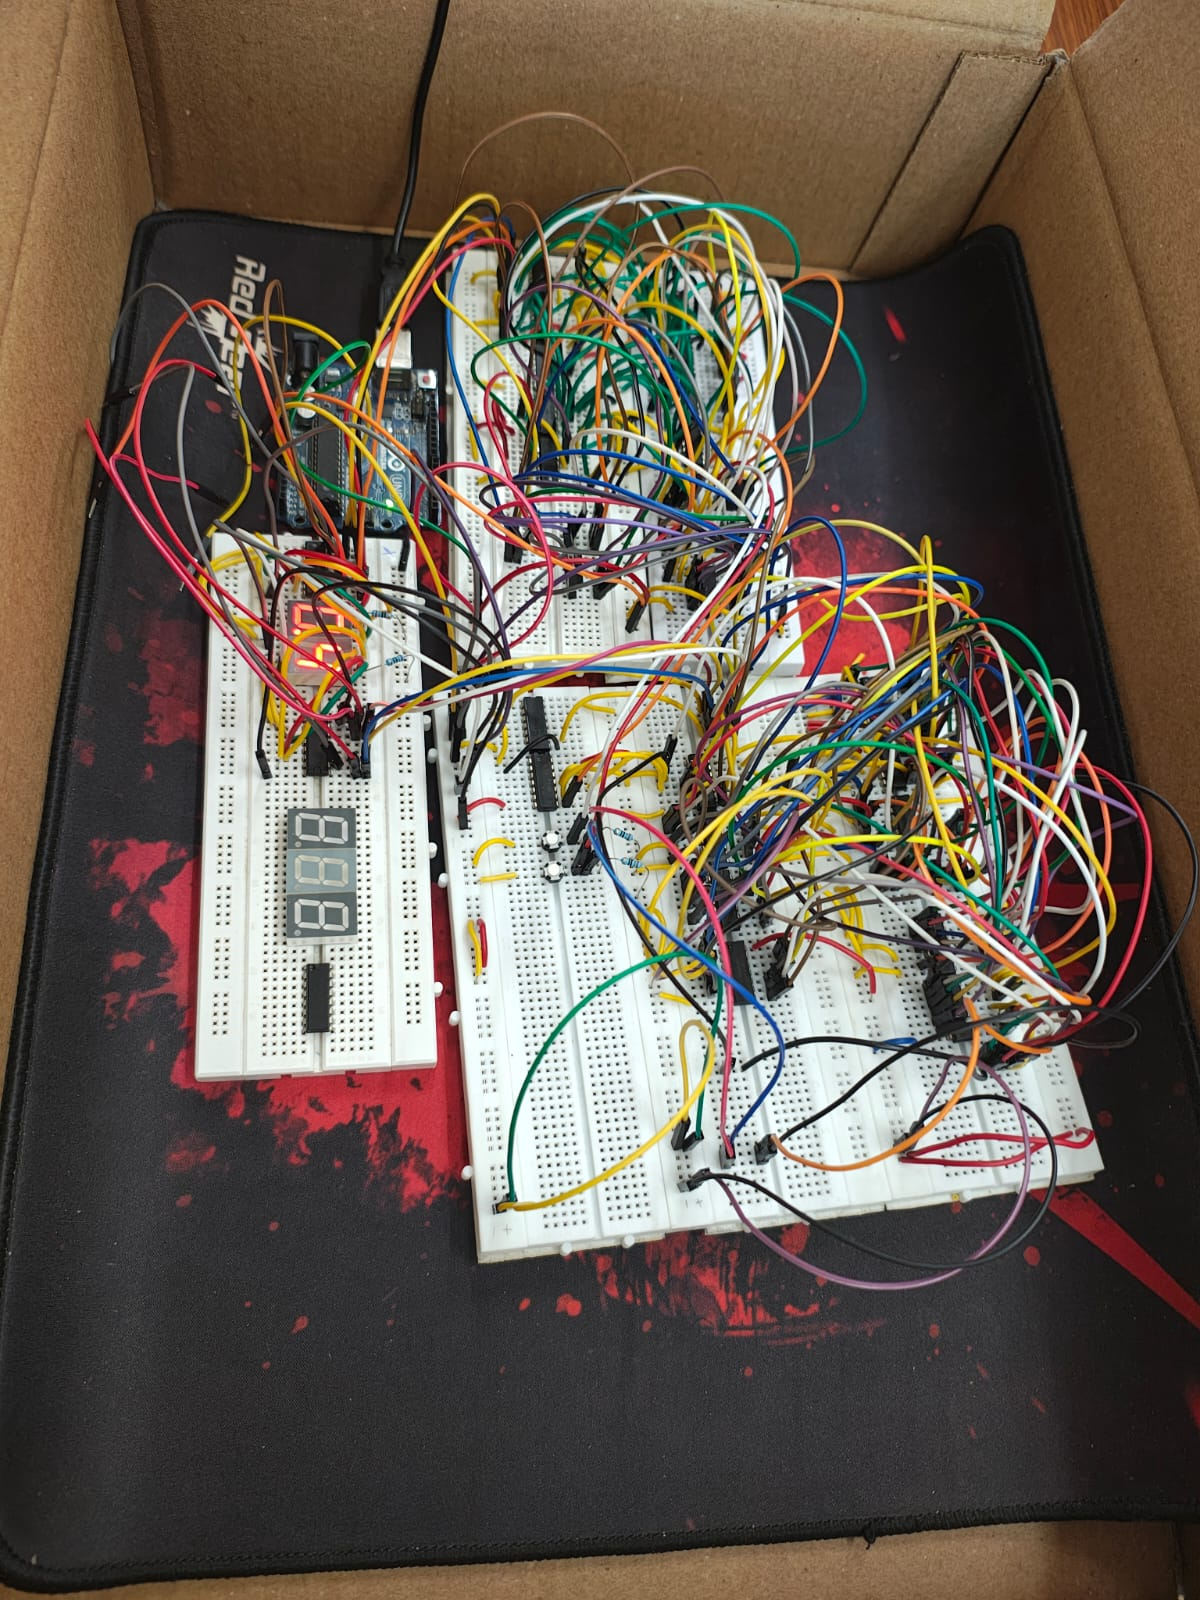
\includegraphics[ width=0.4\textwidth,angle=90]{./figs/image1.jpeg}}
    \hspace{\fill}
    {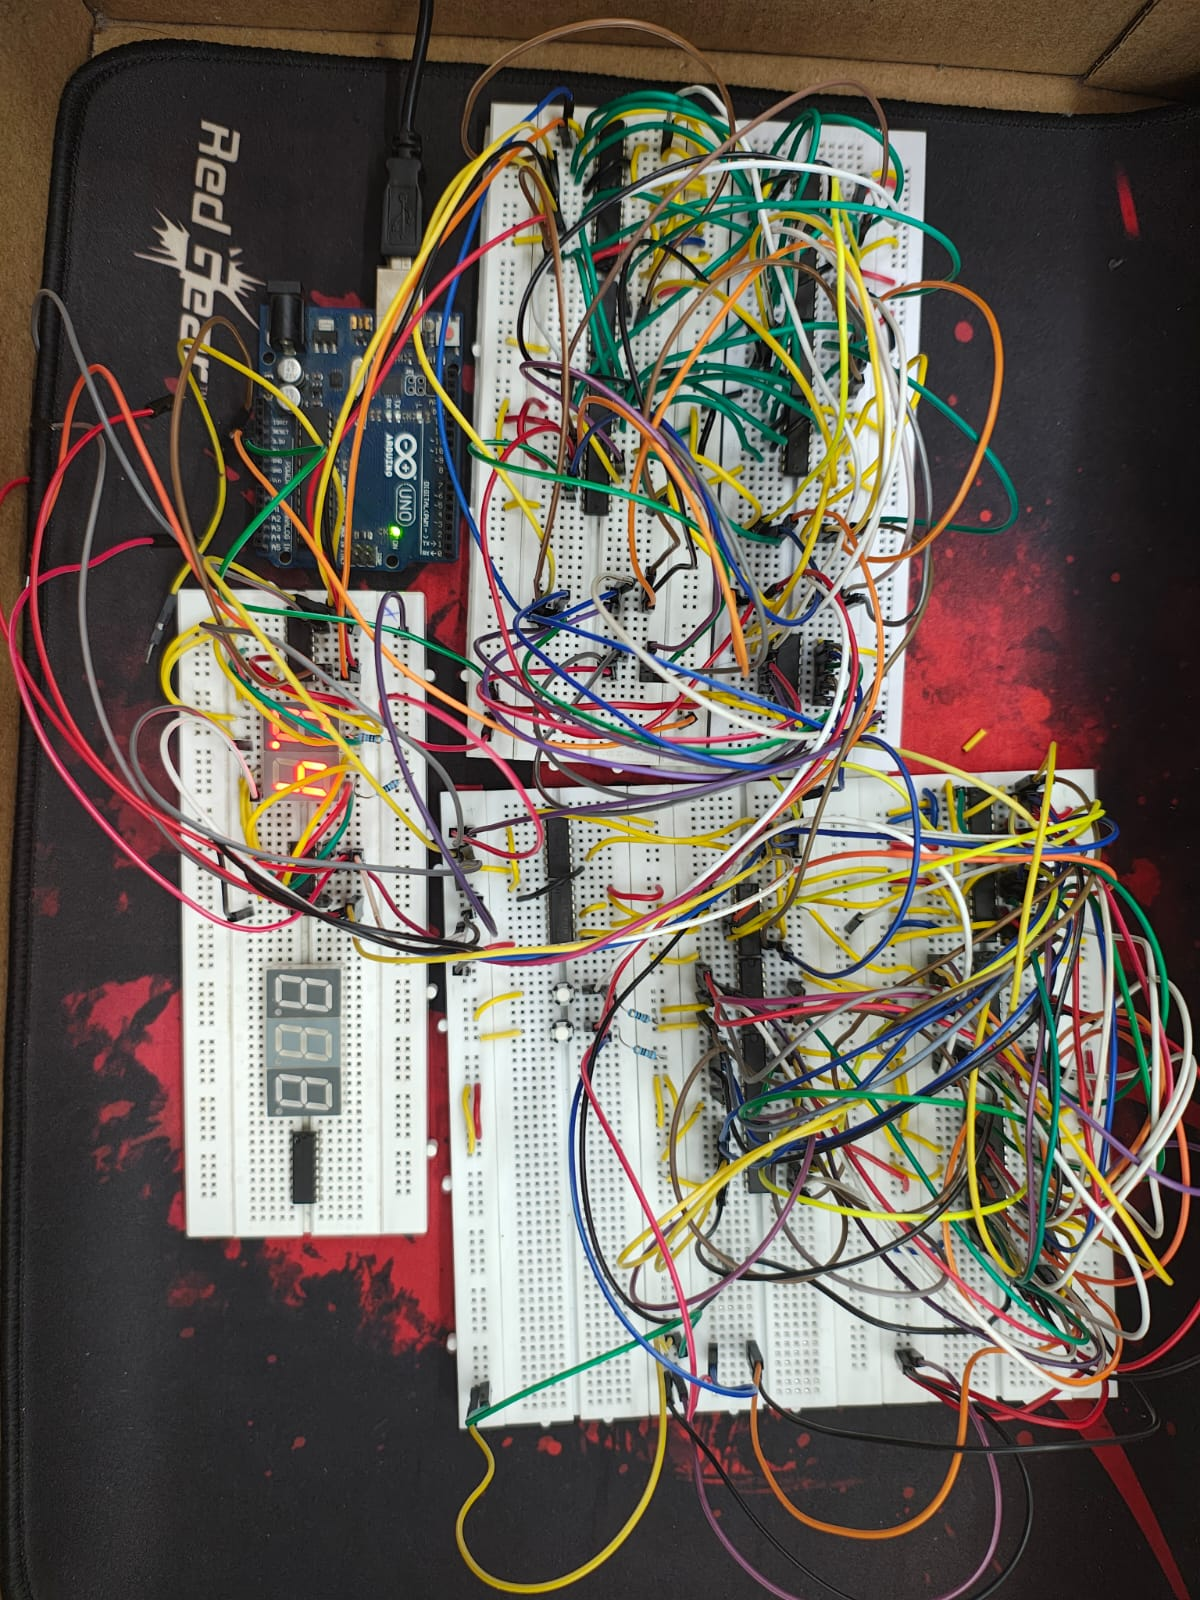
\includegraphics[ width=0.4\textwidth,angle=90]{./figs/image2.jpeg}}
\end{figure*}
\FloatBarrier

\begin{figure*}[!htb]
    {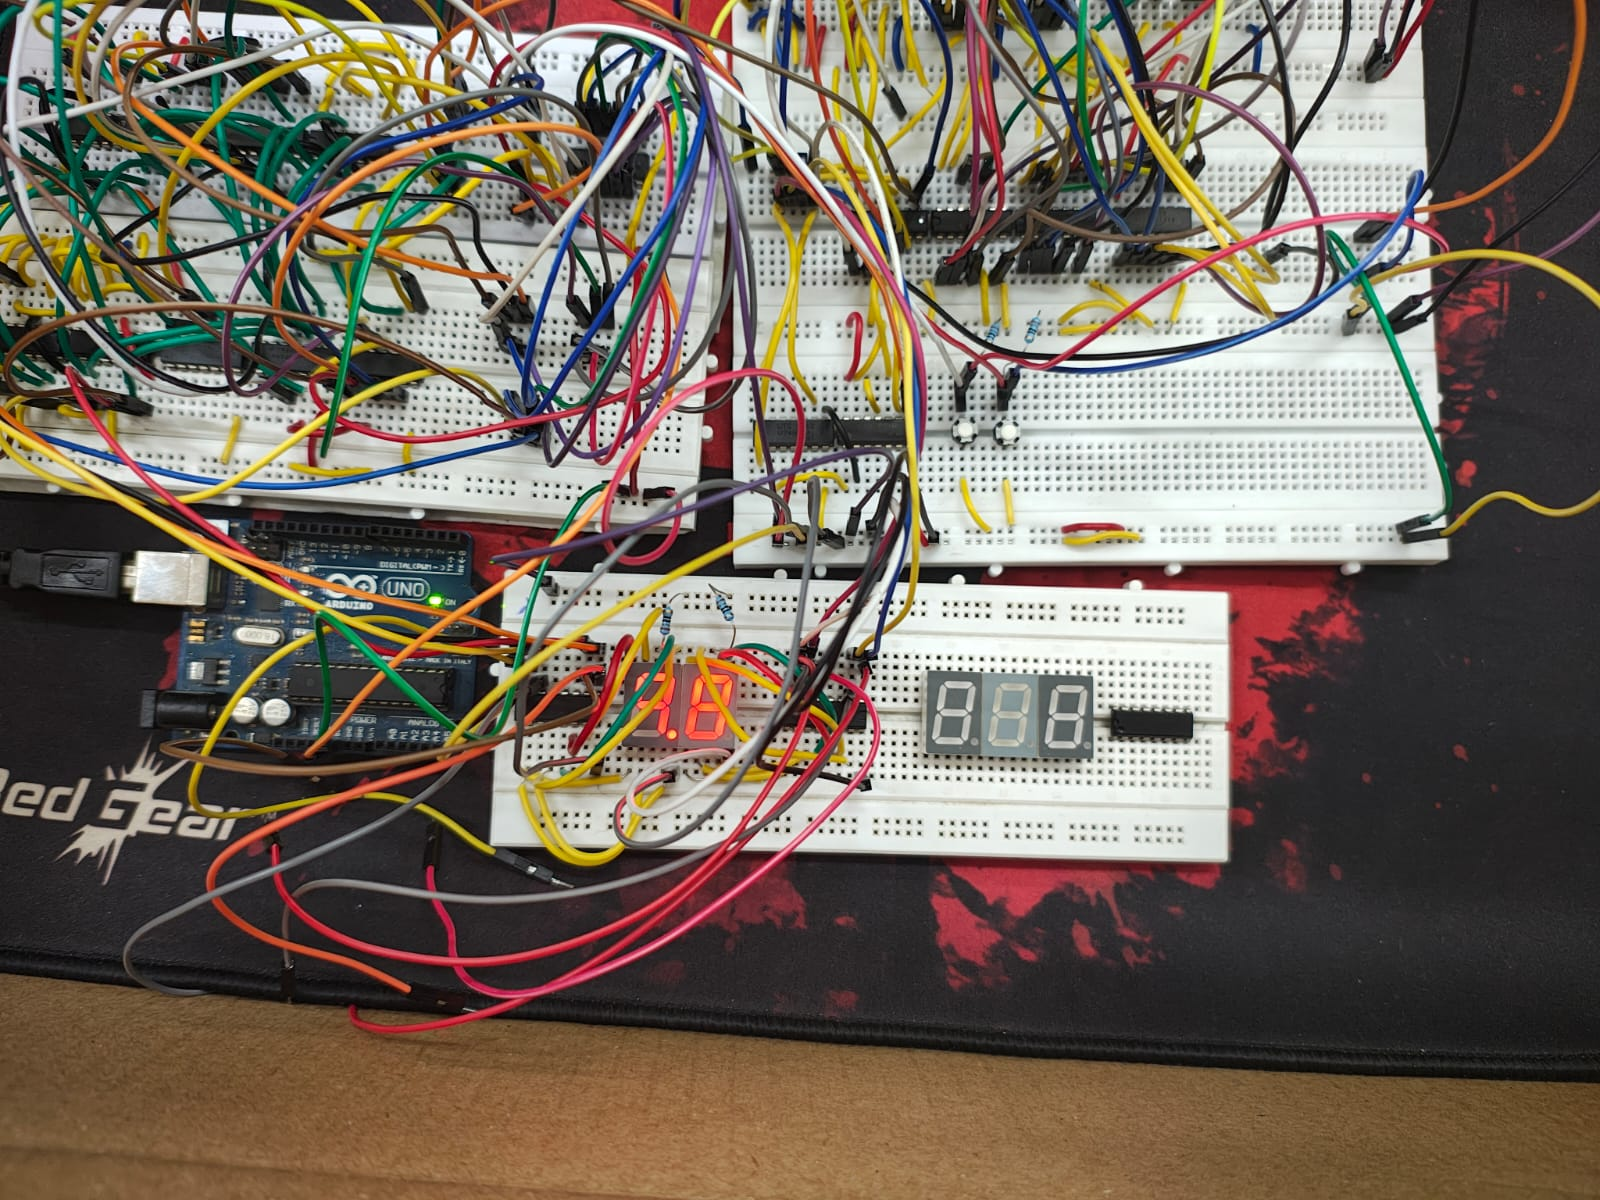
\includegraphics[ width=0.4\textwidth,angle=90]{./figs/image3.jpeg}}
    \hspace{\fill}
    {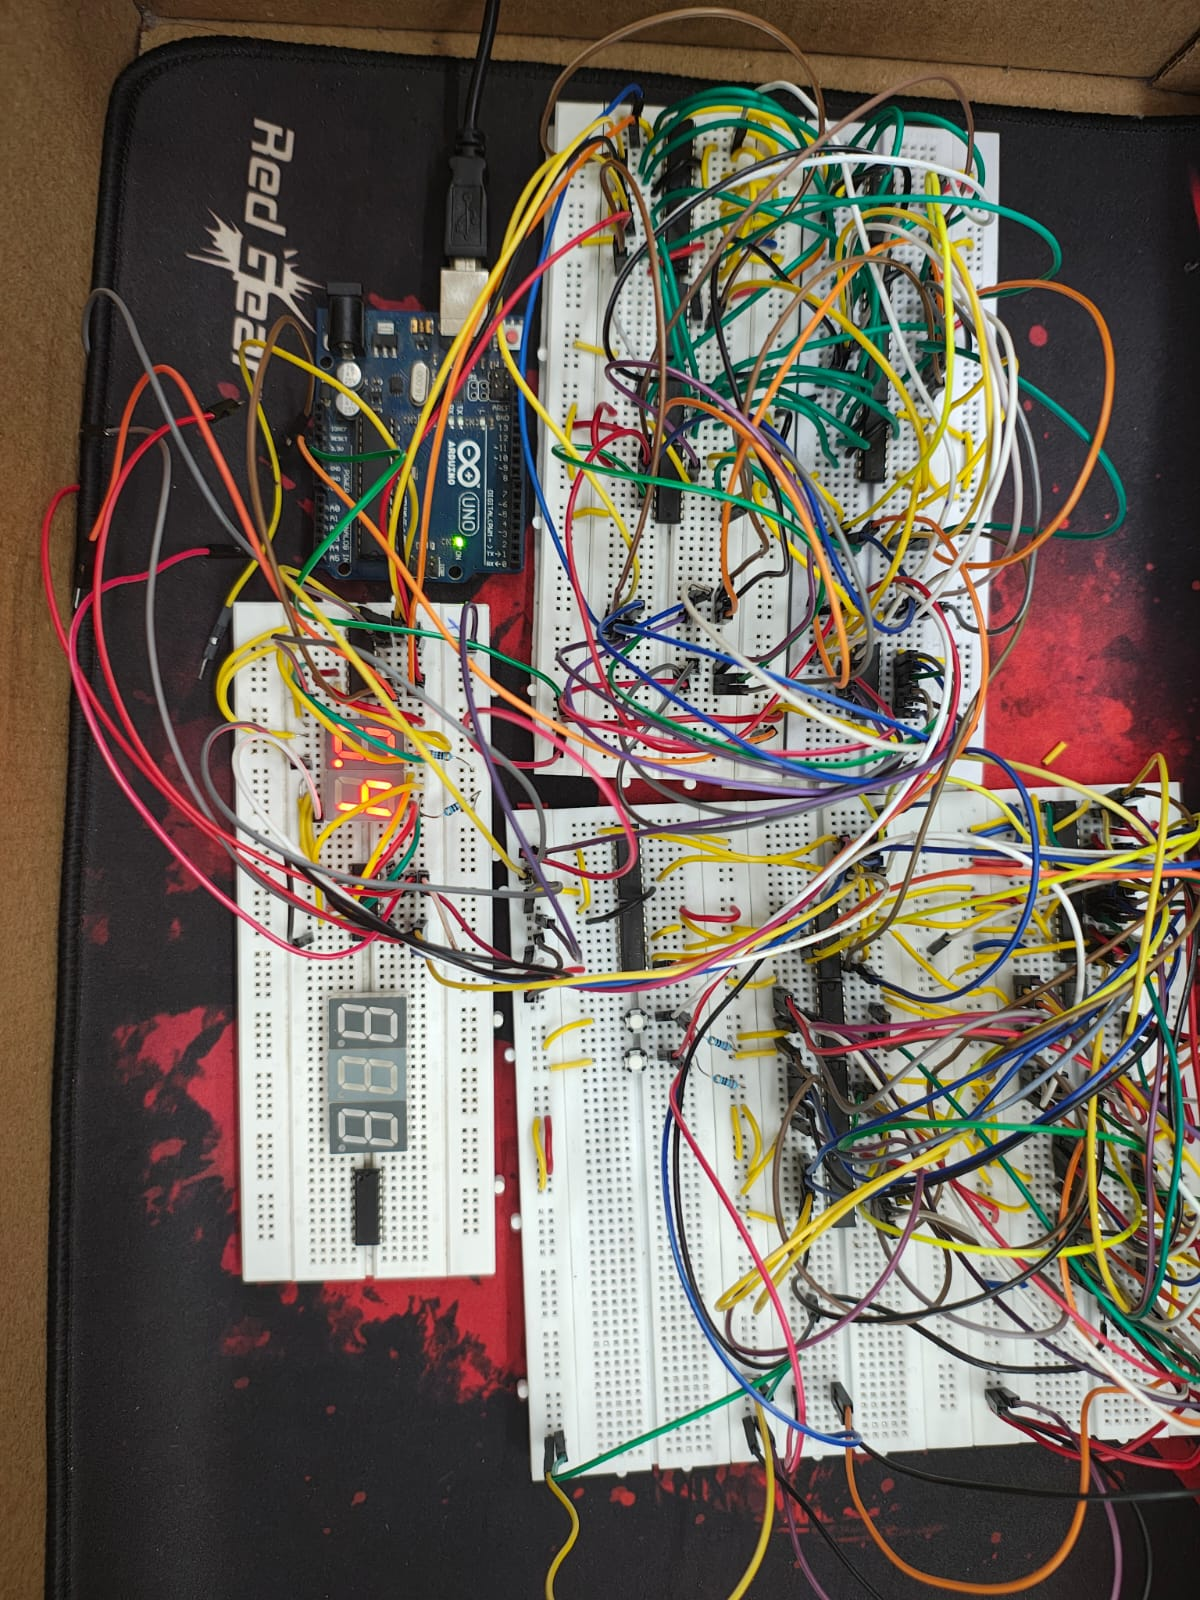
\includegraphics[ width=0.4\textwidth,angle=90]{./figs/image4.jpeg}}
\end{figure*}
\FloatBarrier

\section*{Conclusion}
The BCD counter using T flip-flops was successfully designed and implemented with bidirectional counting capability. The counter correctly counts from 0 to 9 in up mode and from 9 to 0 in down mode, resetting appropriately at the boundaries. The use of push buttons to select the counting direction, along with a BCD-to-7-segment decoder for display, provides a clear demonstration of sequential logic in digital systems. This design can be extended to applications such as digital clocks, frequency counters, and event counters where bidirectional counting is required. The Images and Videos of the Circuit can be found \href{https://github.com/AbhimanyuKoushik/EE1200/tree/main/Lab8/figs}{\textbf{here}}
\end{document}